\documentclass[a4paper,11pt]{article}

\usepackage[portuguese]{babel}
\usepackage[utf8]{inputenc}
\usepackage{amsmath}
\usepackage{graphicx}
\usepackage{hyperref}
\usepackage{float}
\usepackage{subfig}
\usepackage{fixltx2e}
\usepackage[bottom]{footmisc}
\usepackage{listings}
\usepackage{xargs}                      % Use more than one optional parameter in a new commands
\usepackage[pdftex,dvipsnames]{xcolor}  % Coloured text etc.
\usepackage[colorinlistoftodos,prependcaption,textsize=tiny]{todonotes}
\newcommandx{\unsure}[2][1=]{\todo[linecolor=red,backgroundcolor=red!25,bordercolor=red,#1]{#2}}
\newcommandx{\change}[2][1=]{\todo[linecolor=blue,backgroundcolor=blue!25,bordercolor=blue,#1]{#2}}
\newcommandx{\info}[2][1=]{\todo[linecolor=OliveGreen,backgroundcolor=OliveGreen!25,bordercolor=OliveGreen,#1]{#2}}
\newcommandx{\improvement}[2][1=]{\todo[linecolor=Plum,backgroundcolor=Plum!25,bordercolor=Plum,#1]{#2}}
\newcommandx{\thiswillnotshow}[2][1=]{\todo[disable,#1]{#2}}
\usepackage[font=footnotesize]{caption}
\usepackage[hypcap]{caption}
\usepackage[top=2.5cm, bottom=2.5cm, left=2.5cm, right=2.5cm]{geometry}
\usepackage{enumerate}
\usepackage[siunitx,american]{circuitikz}

\setcounter{tocdepth}{3}
\setcounter{secnumdepth}{4}

\numberwithin{equation}{section}
\addto\captionsportuguese{\renewcommand{\contentsname}{Índice}}

\linespread{1.3}
\usepackage{indentfirst}

\begin{document}
\begin{titlepage}
\begin{center}

\hfill \break
\hfill \break


\includegraphics[width=0.3\textwidth]{img/logo}~\\[1cm] 

\textsc{\LARGE Instituto Superior Técnico}\\[0.25cm]
\textsc{\Large Mestrado Integrado em Engenharia Electrotécnica e de Computadores}\\[1.8cm]
\textsc{\huge Electrónica de Potência}\\[0.25cm]

\vspace{6mm}

{\huge \bfseries Conversor CA/CC Monofásico \linebreak Comandado de Meia Onda \\[0.7cm]}
{\bfseries Rectificador de meia onda com carga R e RL \& com carga RL e díodo de roda \\[1cm]}

\begin{tabular}{ l l }
	João Bernardo Sequeira de Sá & \hspace{2mm} n.º 68254 \\
	Maria Margarida Dias dos Reis & \hspace{2mm} n.º 73099 \\
	Rafael Augusto Maleno Charrama Gonçalves & \hspace{2mm} n.º 73786 \\
	Nuno Miguel Rodrigues Machado & \hspace{2mm} n.º 74236
\end{tabular}

\vspace{7mm}

Turno de Segunda-feira das 17h00 - 20h00

\vfill

{\large Lisboa,  de Novembro de 2015} 
	
\end{center}
\end{titlepage}
	
\tableofcontents
\pagebreak

\section{Introdução}

Com este trabalho pretende estudar-se o funcionamento do conversor CA/CC (Retificador) monofásico comandado de meia onda.

Este tipo de retificadores tira o seu nome da capacidade que o tiristor tem em controlar a sua tensão de saída através do ângulo de disparo. O tiristor é levado à condução pela aplicação de um sinal na \textit{gate} e passa ao corte através de comutação natural na maioria dos casos, ou comutação forçada no caso de circuitos fortemente indutivos \cite{Rashid}. 

Pode dizer-se que este trabalho está dividido em duas partes. Na primeira estuda-se o retificador de meia onda simples com carga R e RL. Na segunda parte trata-se da inclusão de um díodo de roda livre e estuda-se o comportamento deste novo circuito de potência com uma carga RL.

O comportamento do retificador de meia onda com uma carga resistiva pura é tal que a corrente e a tensão na carga têm que apresentar a mesma polaridade em qualquer altura. Devido ao comportamento do tiristor apenas existe tensão na saída durante alternâncias positivas, pois quando a corrente se anula no tiristor este passa ao corte, sendo esta característica do comportamento que leva ao nome de ``meia onda''  \cite{Kassakian}.

Já no caso de uma carga RL existe uma ligeira desfasagem entre tensão e corrente, devido à presença da bobine, pelo que a corrente no tiristor apenas se anula quando a tensão já se encontra na sua alternância negativa. Embora continuemos a ter apenas meia onda, já não existe uma distinção certa entre conduzir apenas durante uma das alternâncias \cite{Kassakian}. 

Na segunda parte deste trabalho inclui-se ao circuito um díodo de roda livre. O díodo de roda livre é também conhecido como díodo \textit{snubber} ou díodo \textit{flyback} \cite{Silva}. Este é utilizado para prevenir valores negativos de tensão na saída assim como eliminar os picos de tensão quando se têm cargas indutivas a sofrer comutação \cite{Kassakian}. 



\section{Condução do Trabalho}

\subsection{Estudo do circuito de disparo}

O circuito de disparo utilizado neste trabalho pode ser representado por um diagrama de blocos tal como se observa na \autoref{fig:circuit_1}.

Como este está preparado para servir como circuito de disparo para um retificador de ponte completa, inclui a capacidade de realizar o \textit{trigger} de 4 tiristores, sendo estes disparados aos pares e consecutivamente. O circuito é constituído por um transformador que amostra a tensão de entrada (TR\_SINC), garantindo a sincronia entre a geração dos impulsos e a tensão; um circuito integrado (UAA145), que detecta a passagem da tensão da rede por zero e gera impulsos em $\alpha$ e $\alpha + \pi$ e um circuito integrado (NE555) e duas portas lógicas NAND, que combinam os impulsos num trem e garantem que a potência da \textit{gate} dos tiristores não é excedida.

\begin{figure}[h]
	\centering
	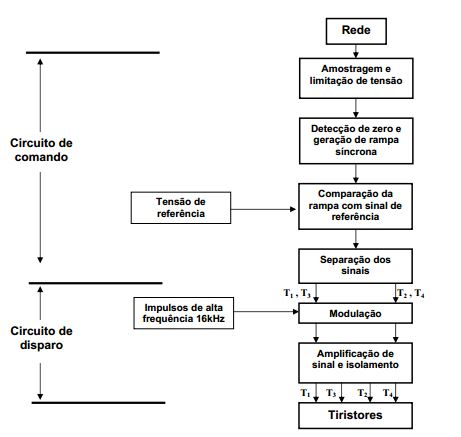
\includegraphics[keepaspectratio=true, scale=0.8]{teoricas/circuito_disparo}
	\caption{Diagrama de blocos do circuito de disparo.}
	\label{fig:circuit_1}
	\vspace{-0.8em}
\end{figure}

\subsubsection{Formas de onda dos sinais de disparo}

Para que fosse possível estudar o funcionamento do circuito de disparo começou por se observar as formas de onda da tensão amostrada de entrada e dos impulsos gerados.

\begin{figure}[H]
	\centering
	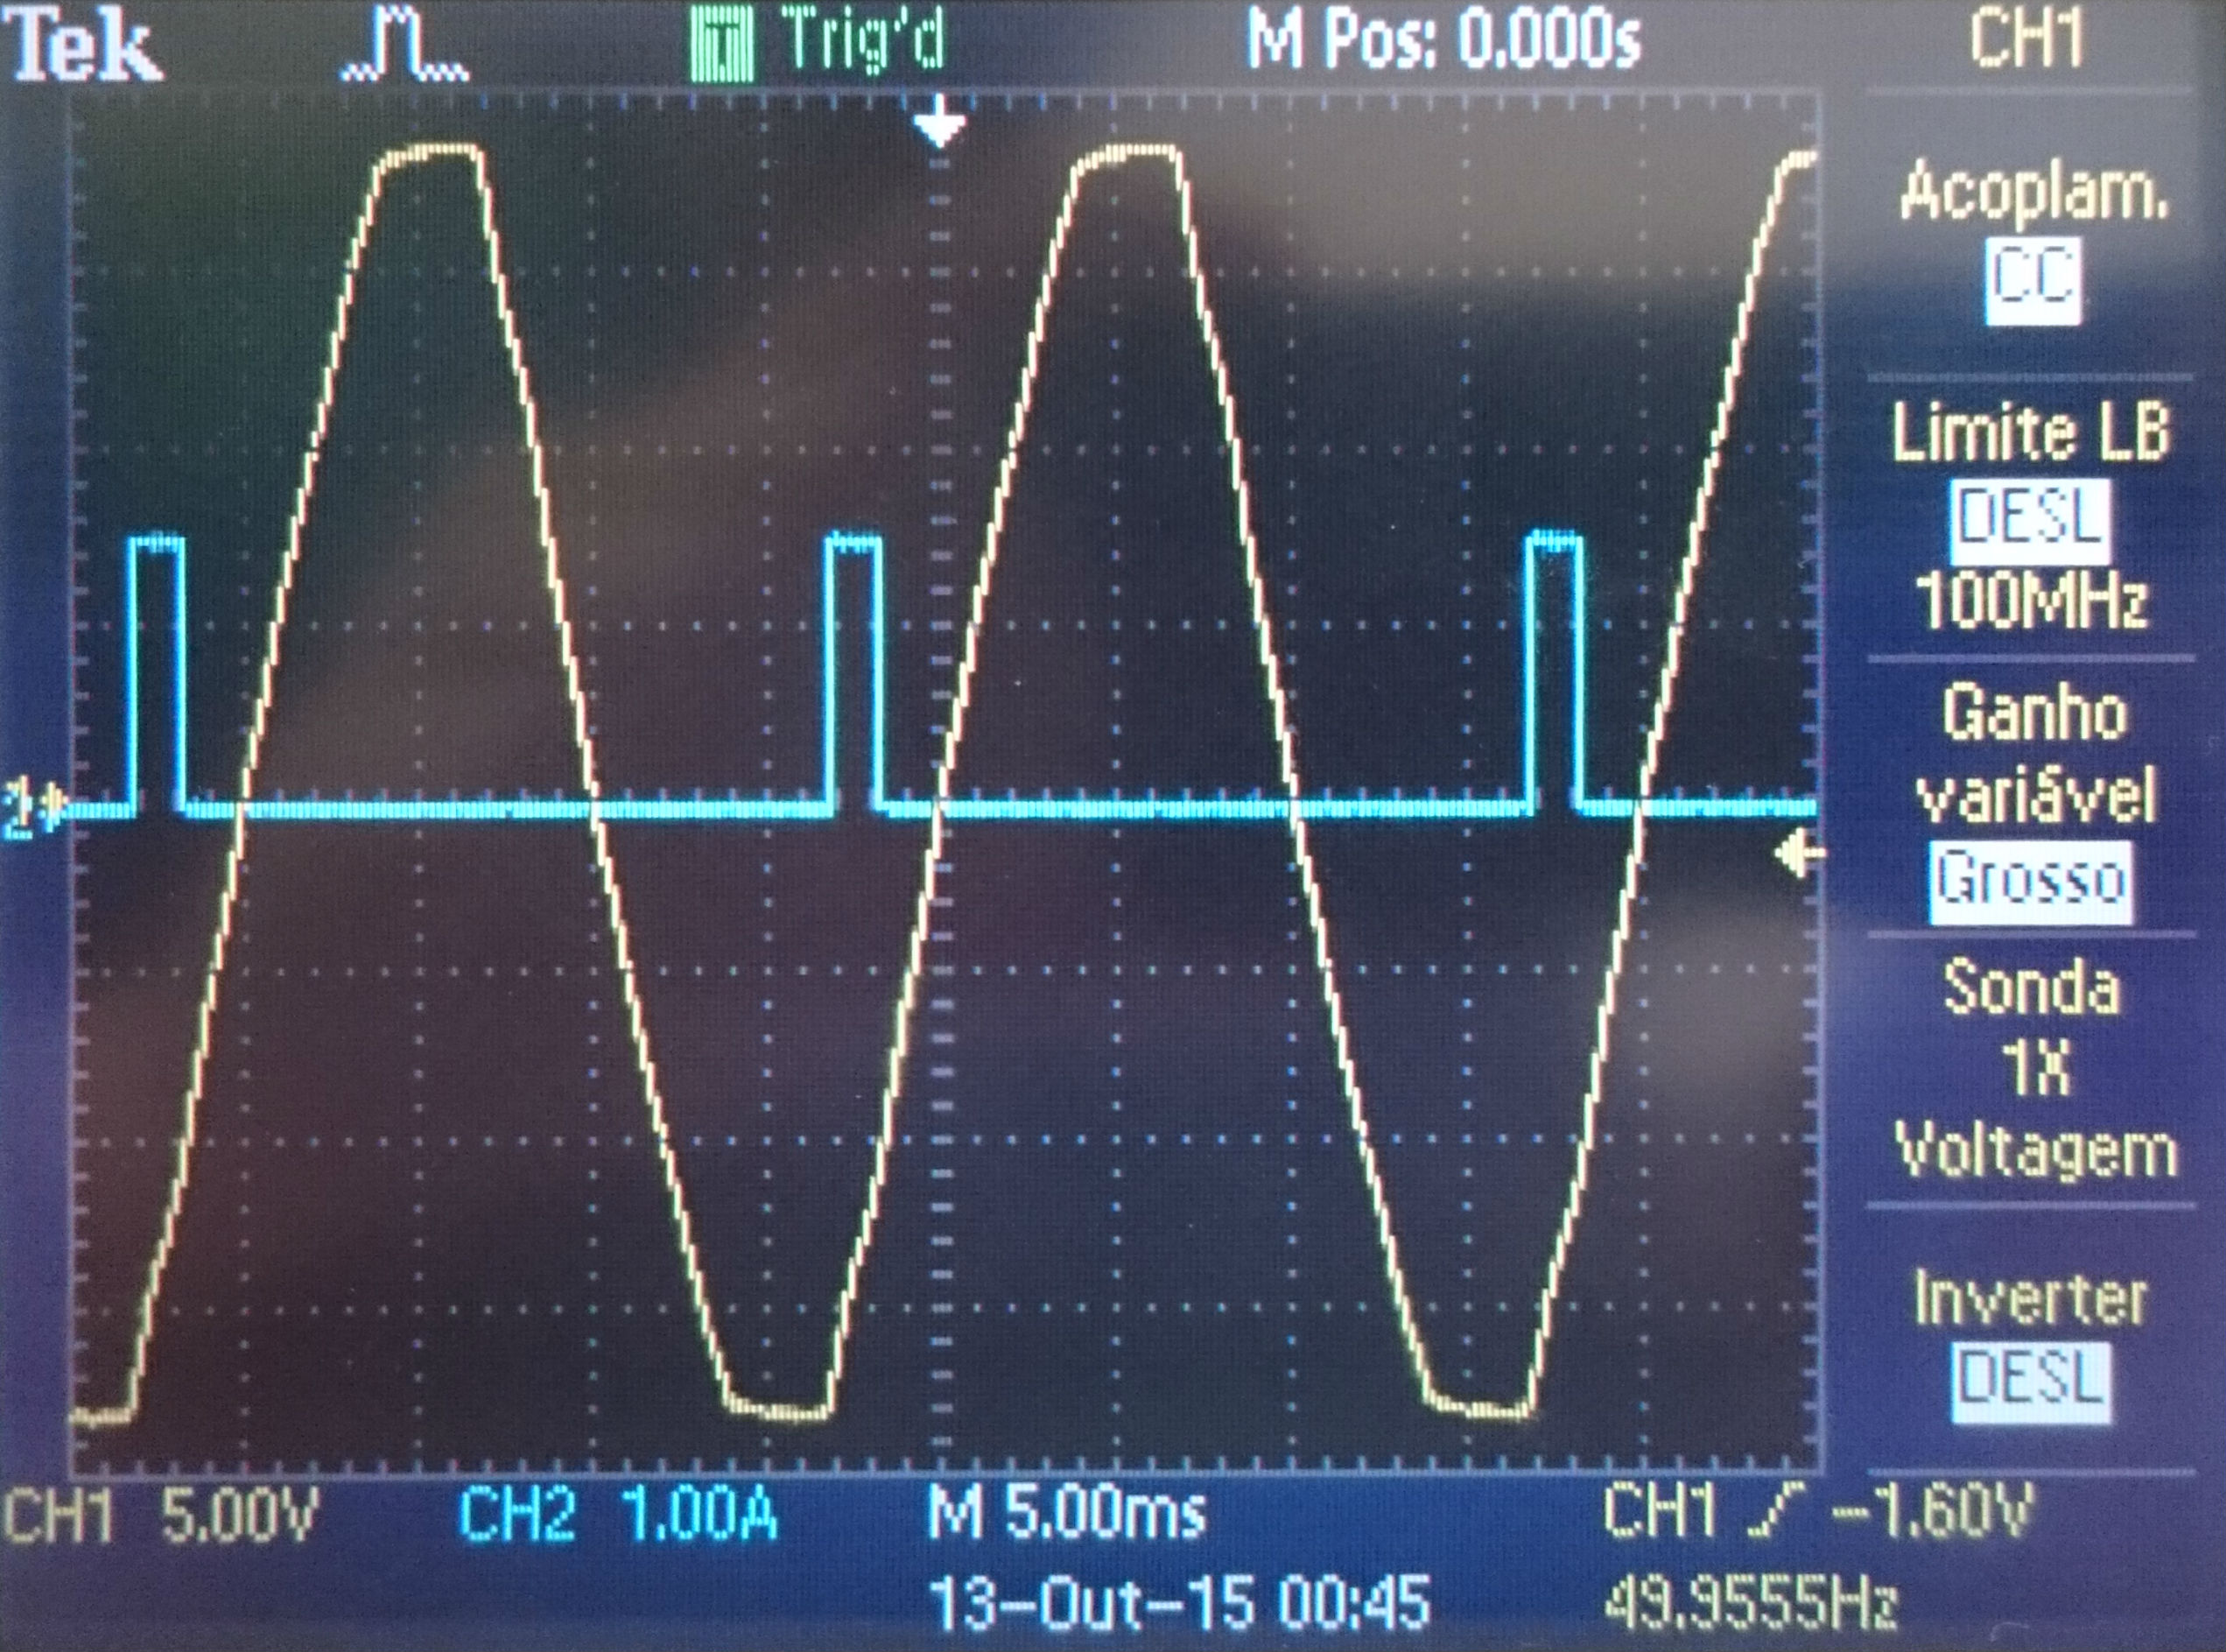
\includegraphics[keepaspectratio=true, scale=0.11]{img/figs/AB_1}
	\caption{Forma de onda da tensão em A e B.}
	\label{fig:AB_1}
	\vspace{-0.8em}
\end{figure}

\begin{figure}[H]
	\centering
	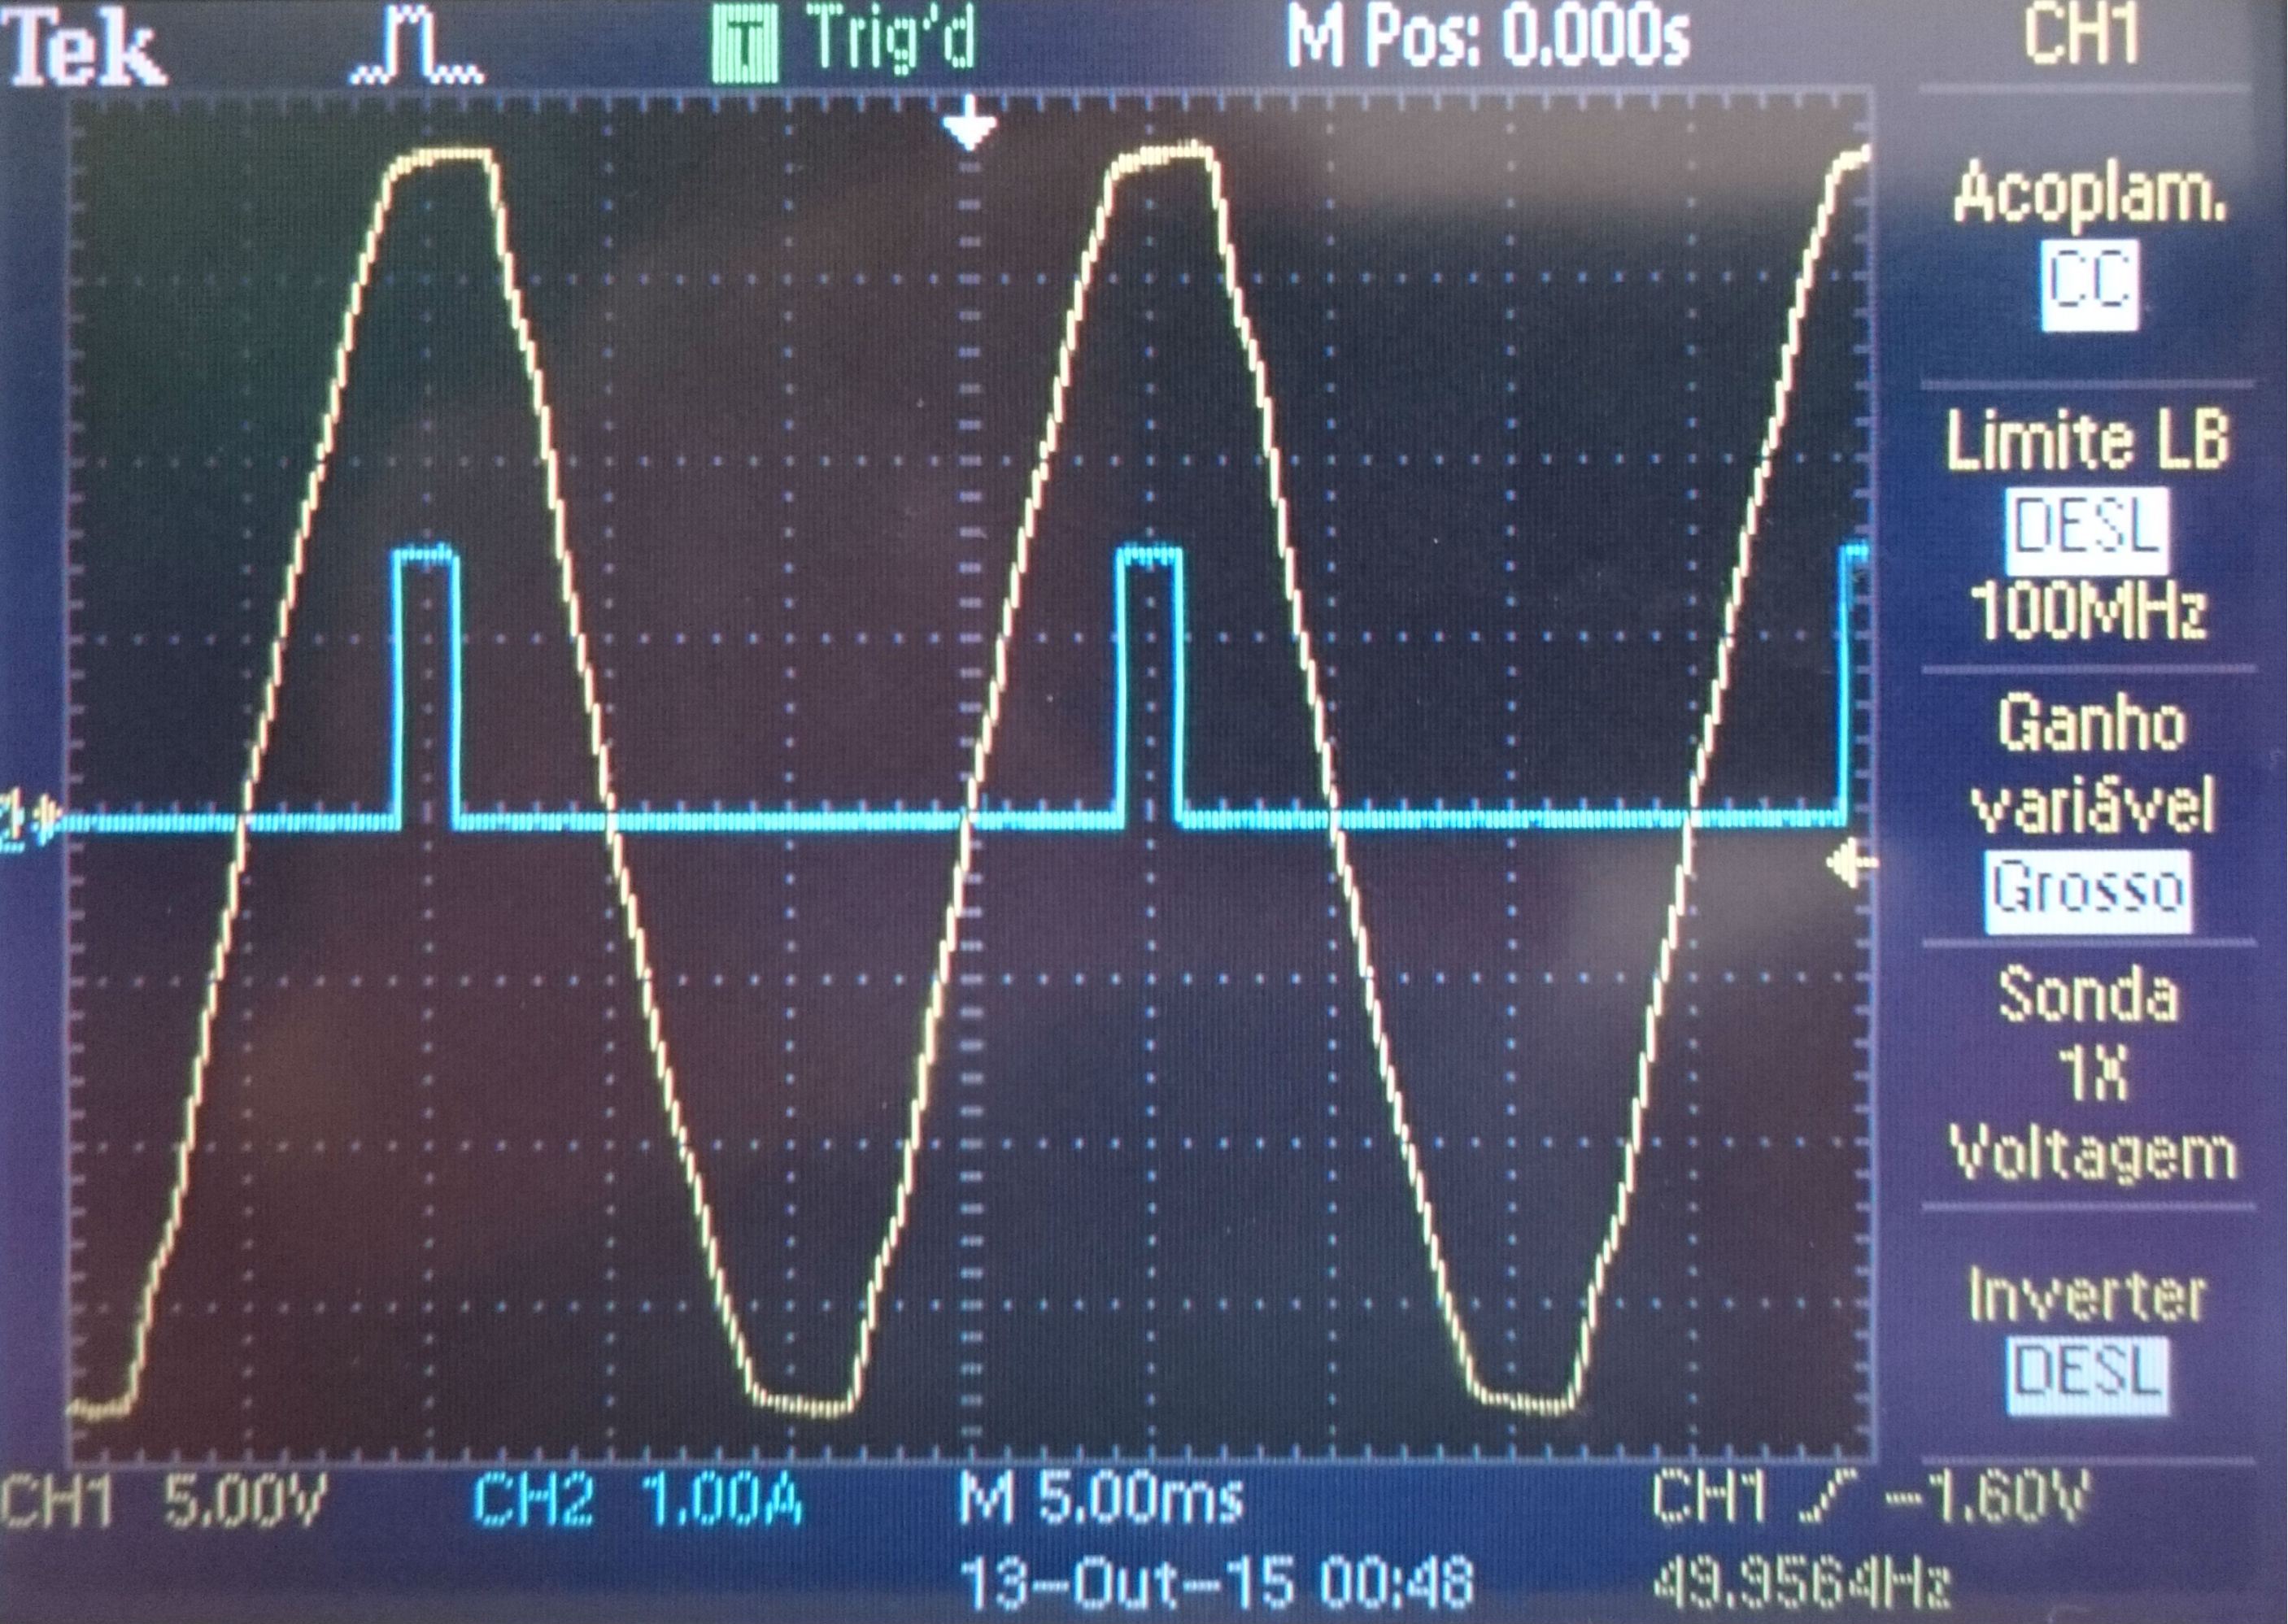
\includegraphics[keepaspectratio=true, scale=0.1]{img/figs/AC_1}
	\caption{Forma de onda da tensão em A e C.}
	\label{fig:AC_1}
	\vspace{-0.8em}
\end{figure}

Na \autoref{fig:AB_1} pode ver-se a amarelo a tensão amostrada pelo transformador e a azul o impulso de \textit{trigger} gerado para $\alpha$. Já na \autoref{fig:AC_1} pode observar-se a amarelo novamente a tensão amostrada e a azul o impulso de \textit{trigger} gerado para $\alpha + \pi$.

A posição destes dois impulsos pode ser controlada através do valor do ângulo de disparo $\alpha$ manipulando um potenciómetro presente na placa do circuito de disparo. Ao mudar este valor, as formas de onda são observáveis, tanto para a tensão amostrada e o impulso $\alpha$ como para a mesma tensão e o impulso  $\alpha + \pi$, na \autoref{fig:AB_2} e \autoref{fig:AC_2} respectivamente.

\begin{figure}[H]
	\centering
	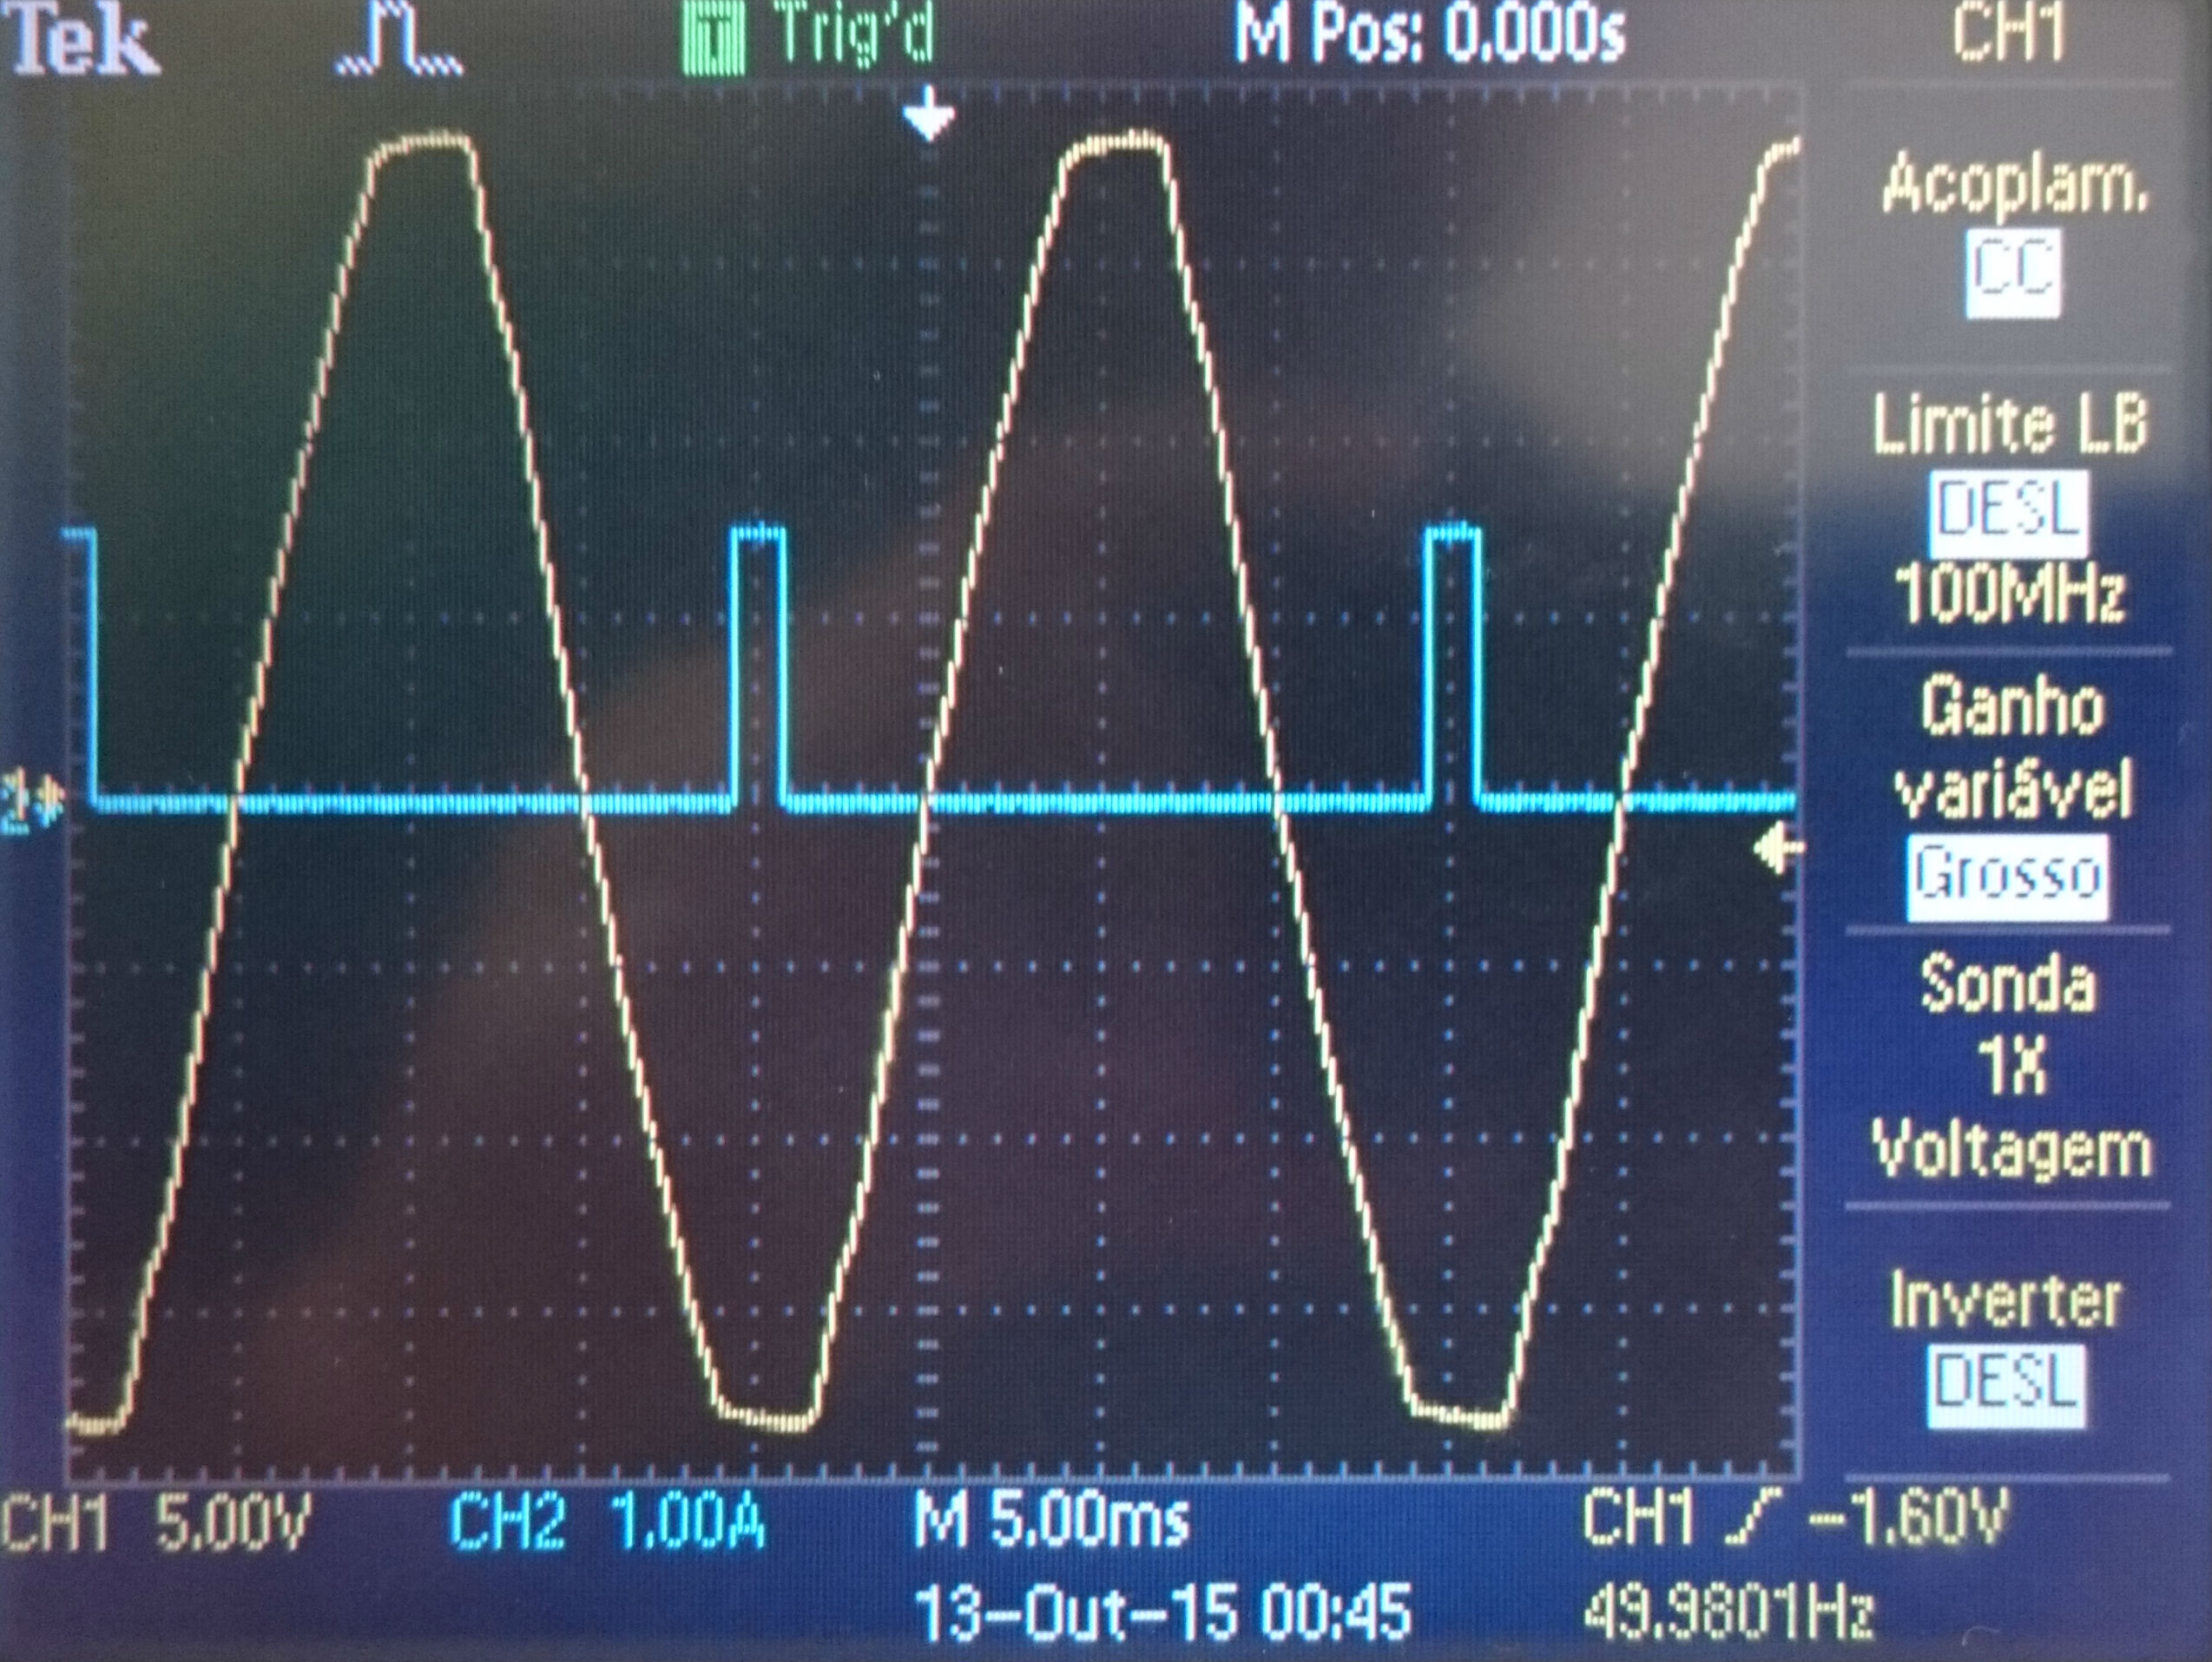
\includegraphics[keepaspectratio=true, scale=0.11]{img/figs/AB_2}
	\caption{Forma de onda da tensão em A e B para novo $\alpha$.}
	\label{fig:AB_2}
	\vspace{-0.8em}
\end{figure}

\begin{figure}[H]
	\centering
	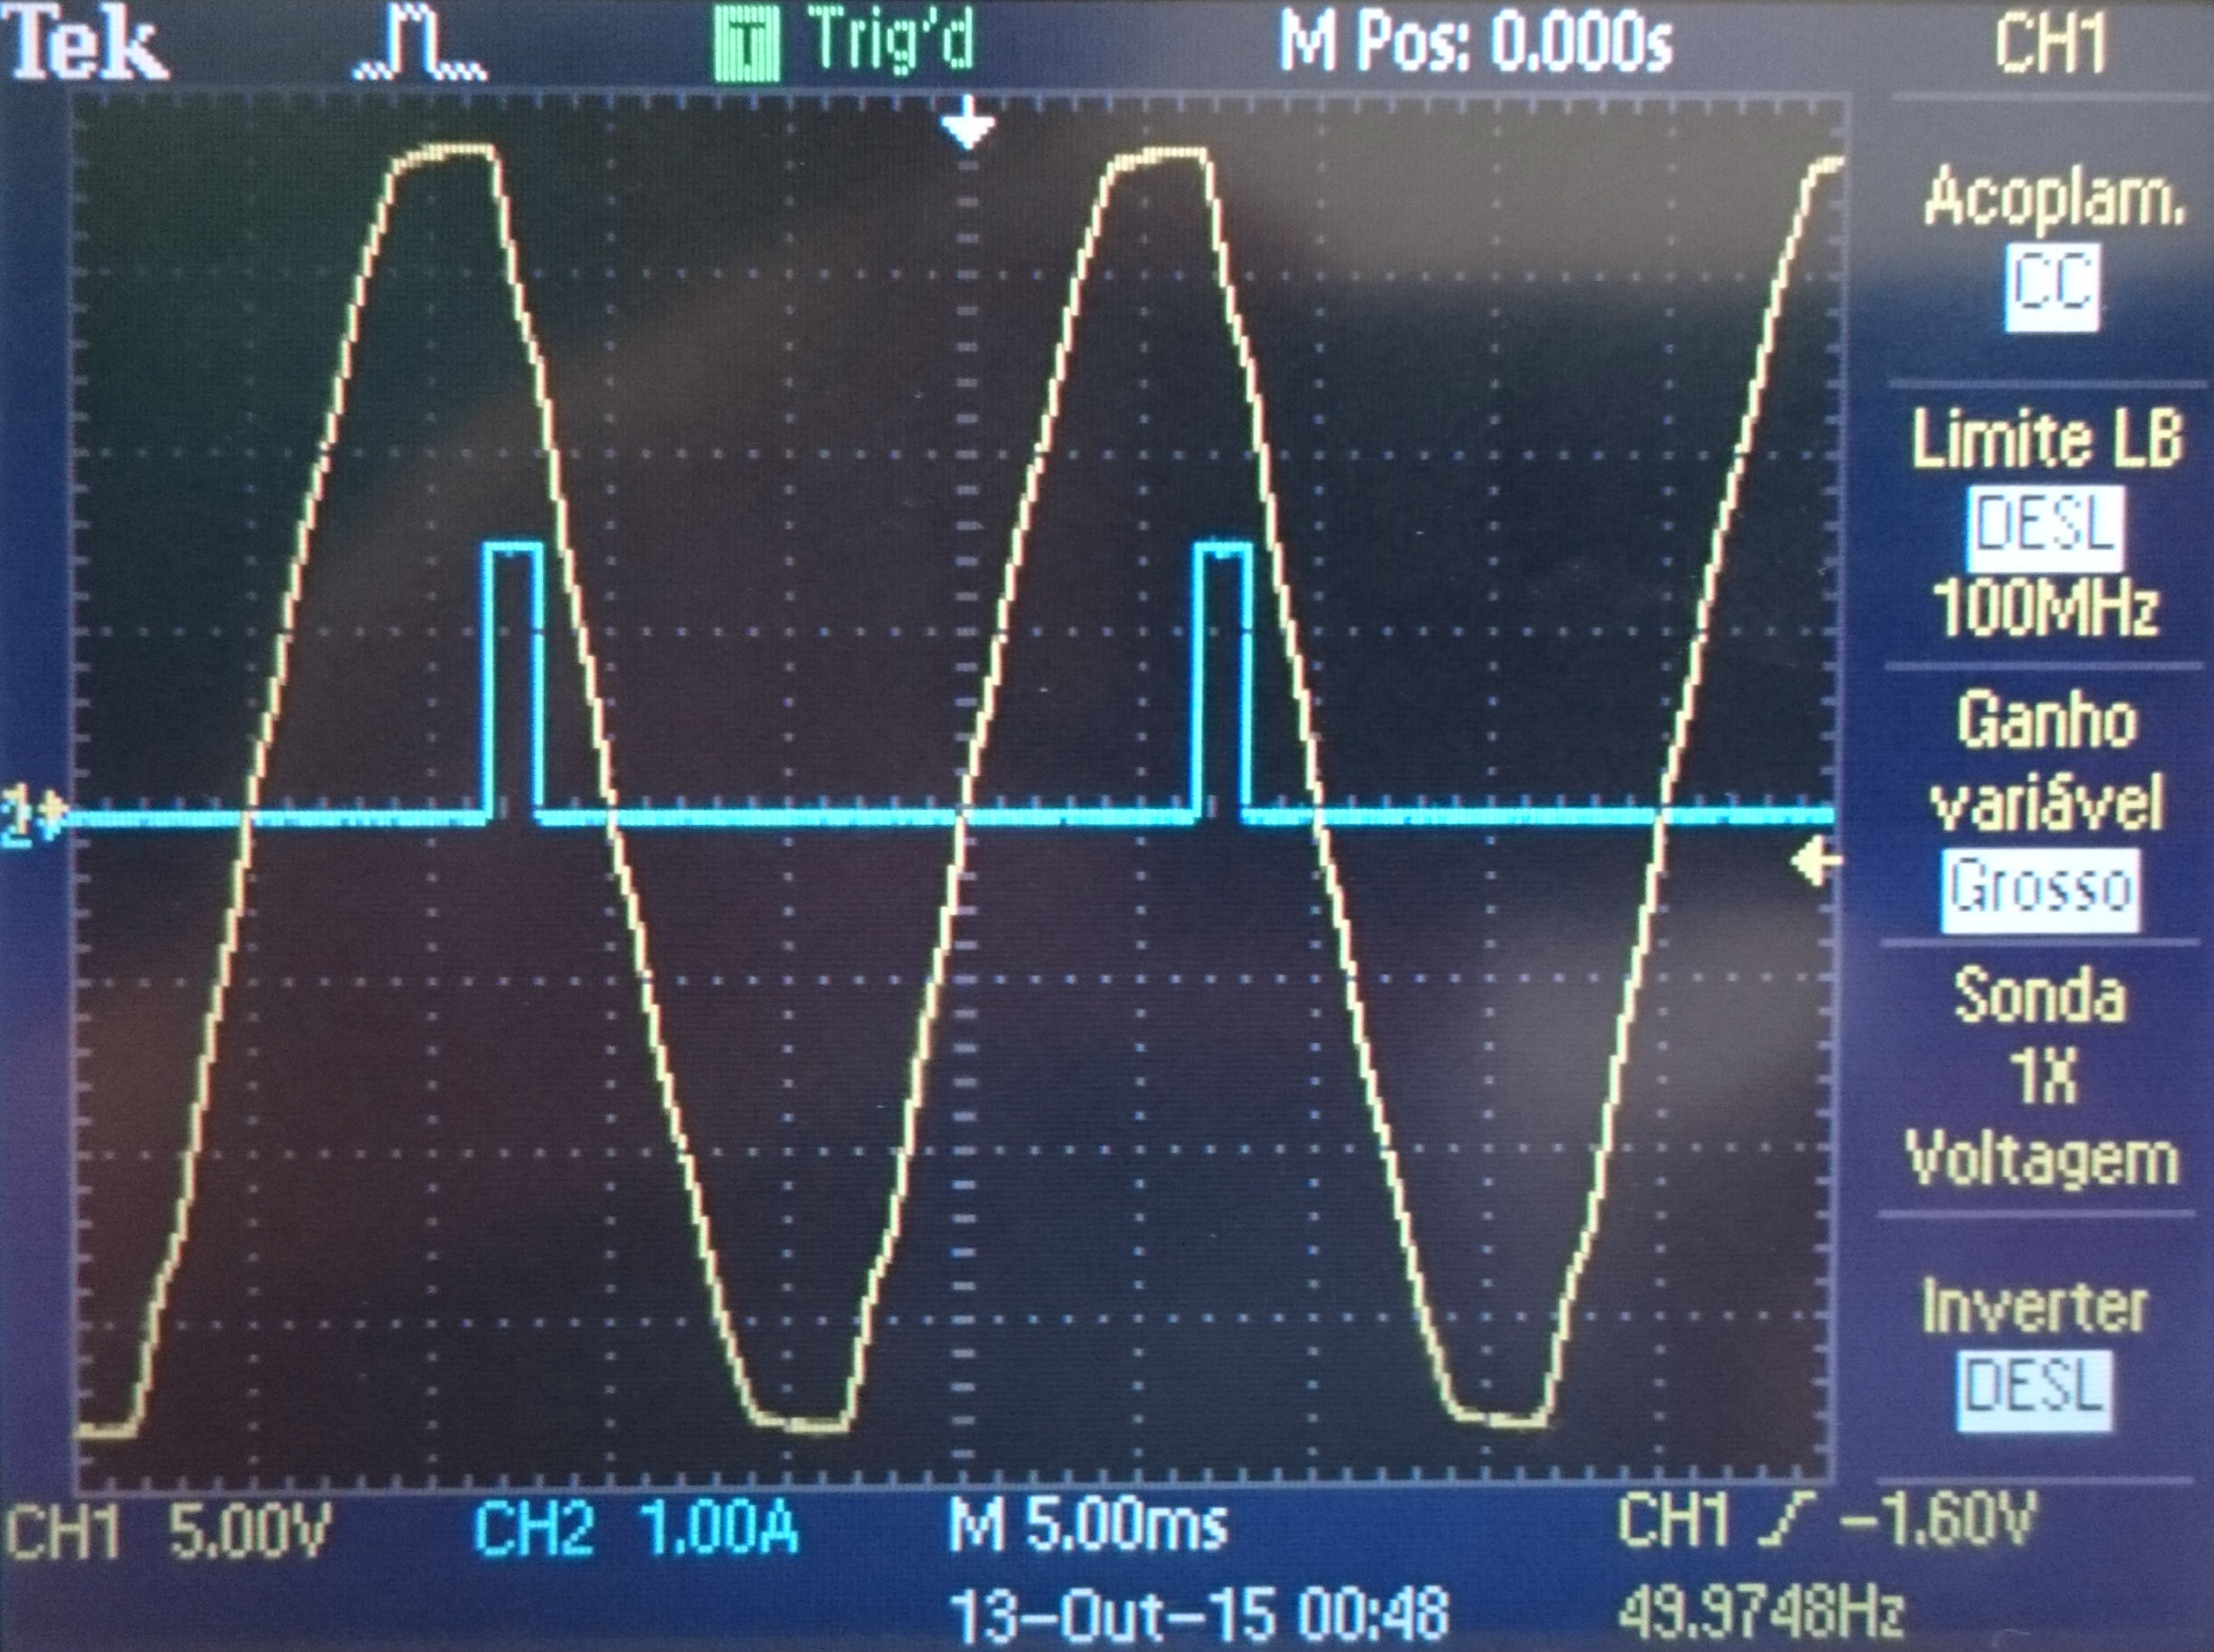
\includegraphics[keepaspectratio=true, scale=0.11]{img/figs/AC_2}
	\caption{Forma de onda da tensão em A e C para novo $\alpha$.}
	\label{fig:AC_2}
	\vspace{-0.8em}
\end{figure}


\subsubsection{Trem de impulsos}

Como a frequência de operação é a da rede, $50$ Hz, os impulsos de disparo devem ter durações de poucos milissegundos, evitando-se efeitos negativos de \textit{latching}, sendo estes especialmente prevalentes no caso de cargas indutivas em que o ângulo de disparo será elevado. No entanto estas durações podem saturar o transformador de impulsos ou provocar perdas elevadas na \textit{Gate} do Tiristor.

Para resolver ambos estes problemas utiliza-se um trem de impulsos de \textit{trigger}.

\begin{figure}[H]
	\centering
	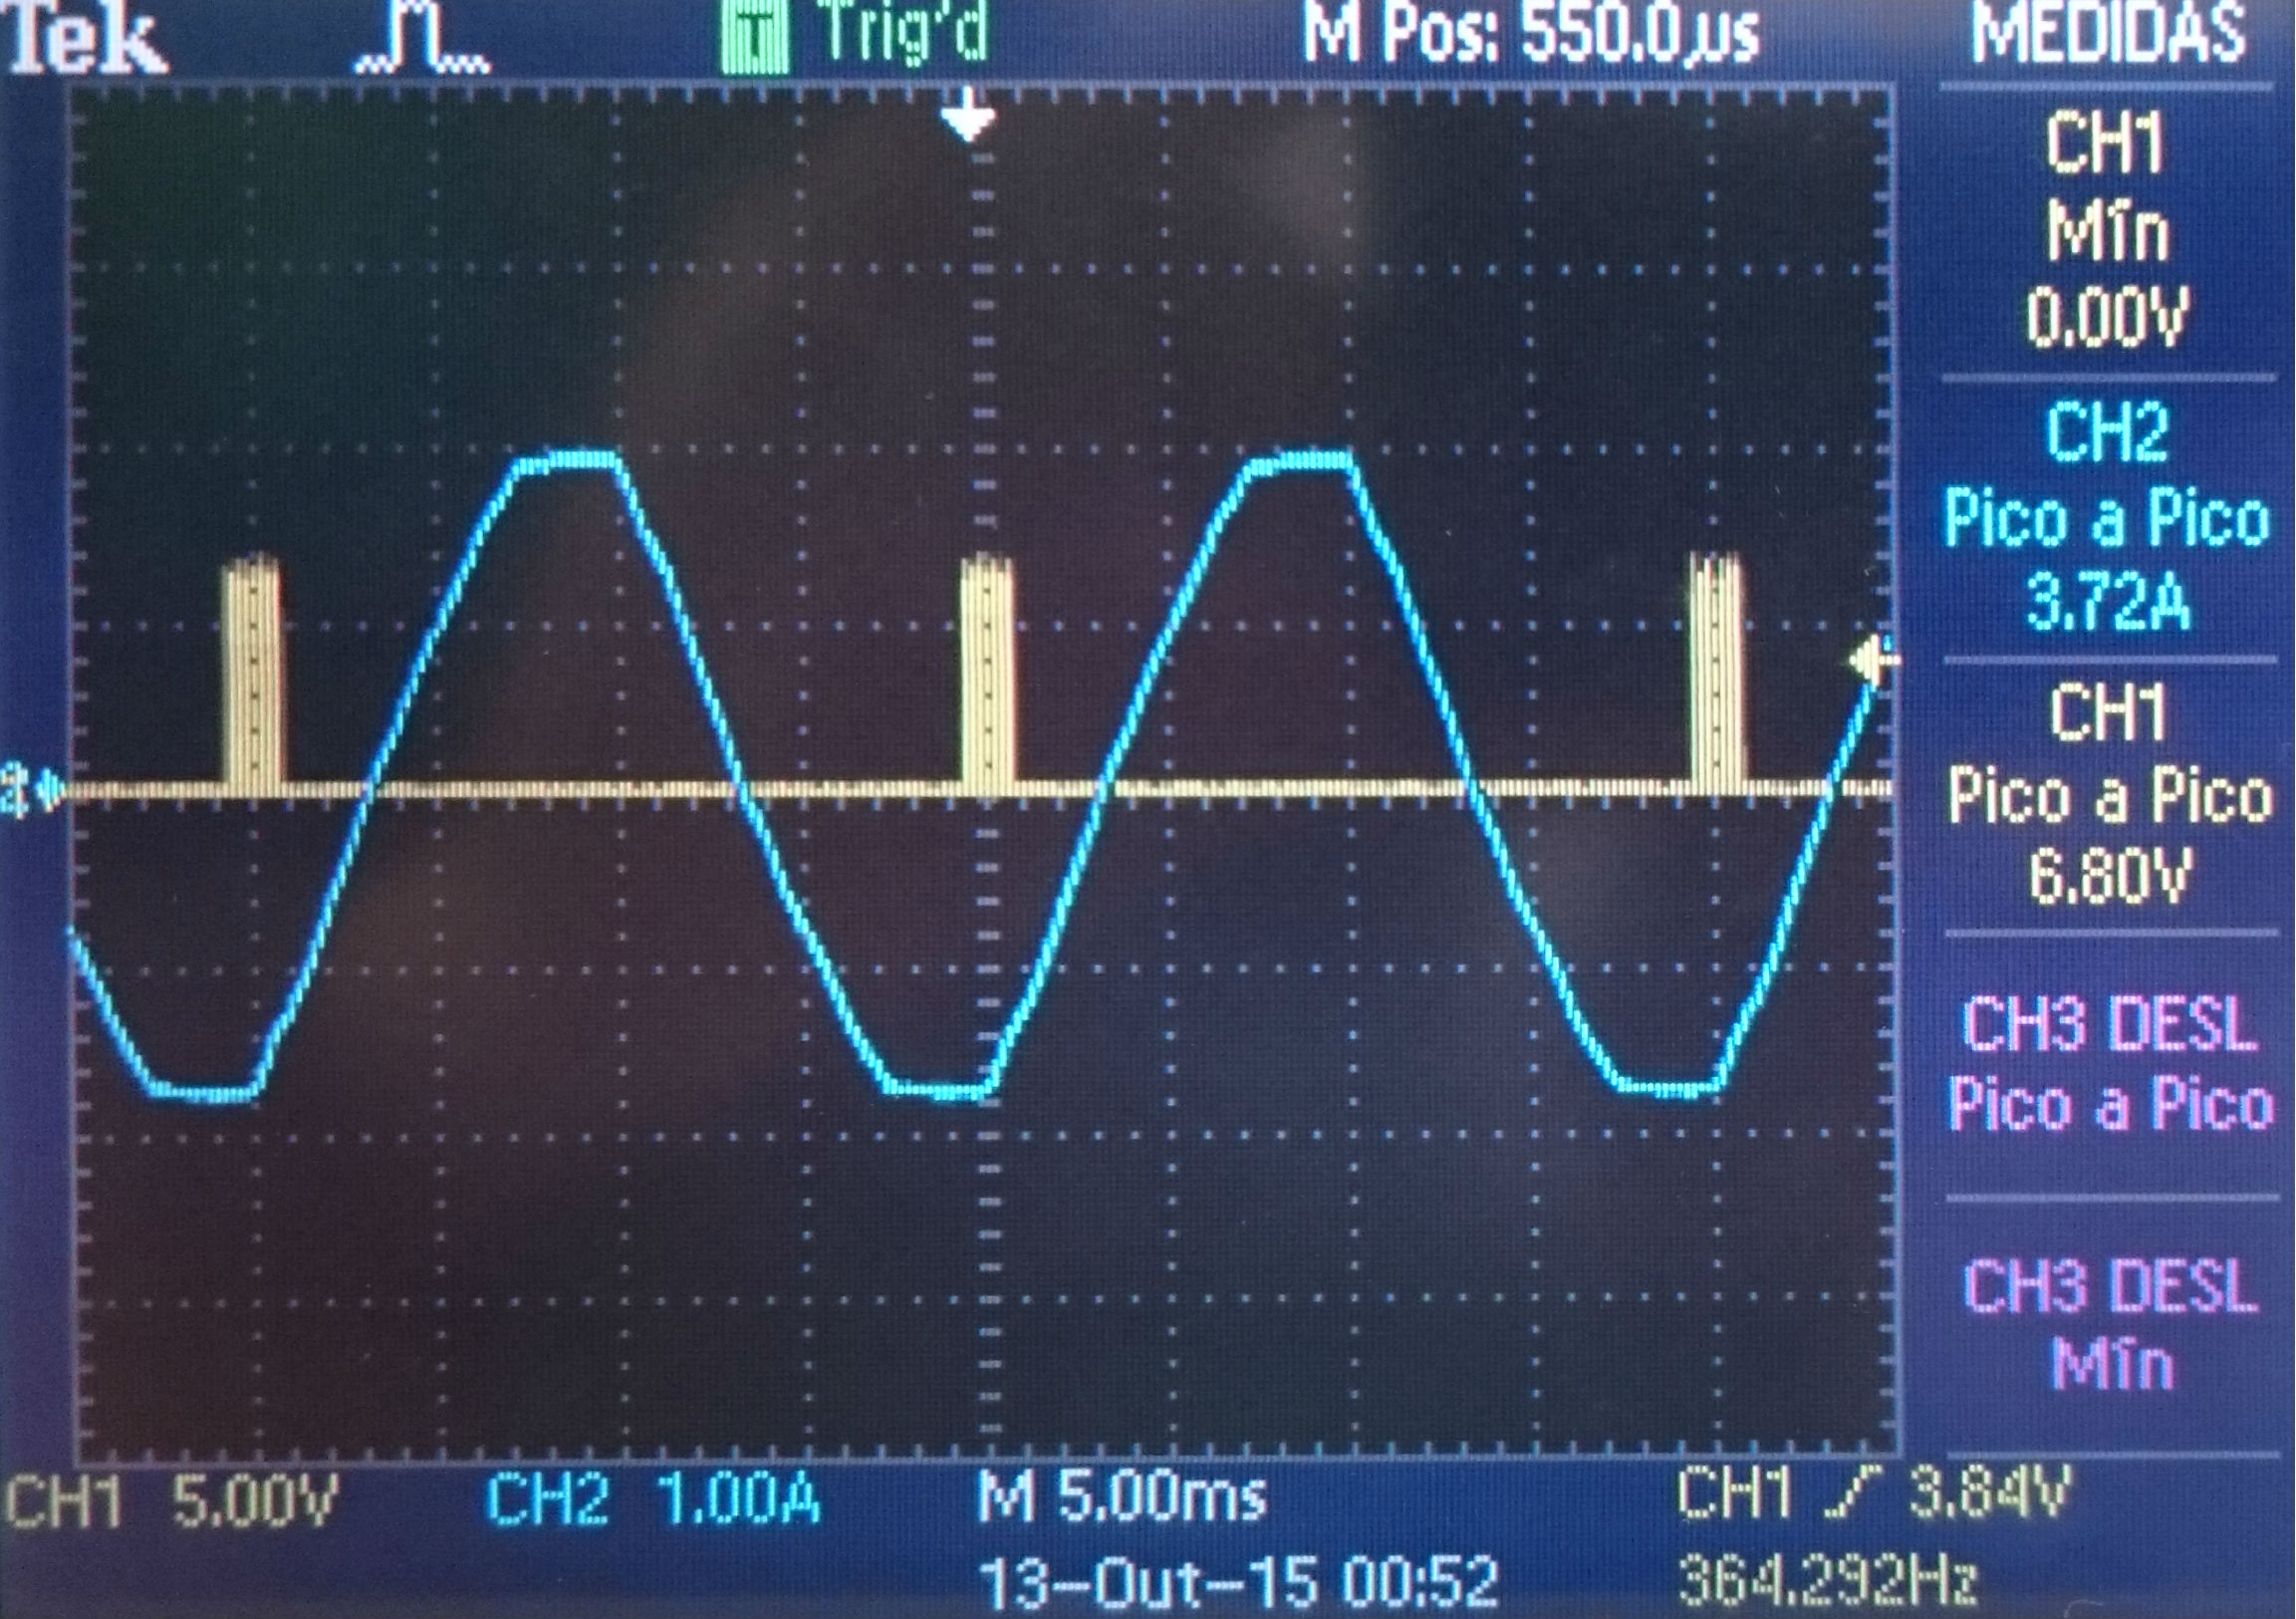
\includegraphics[keepaspectratio=true, scale=0.115]{img/figs/trem_impulsos_A}
	\caption{Formas de onda do trem de impulso e tensão em A.}
	\label{fig:trem_impulsos_A}
	\vspace{-0.8em}
\end{figure}

Colocou-se entre a ``\textit{gate}'' e o cátodo do circuito de controlo uma resistência de $33$ $\Omega$ para simular a \textit{gate} do tiristor. Na \autoref{fig:trem_impulsos_A} pode assim ver-se a azul a queda de tensão nessa resistência e a amarelo o trem de impulsos.

\begin{figure}[H]
	\centering
	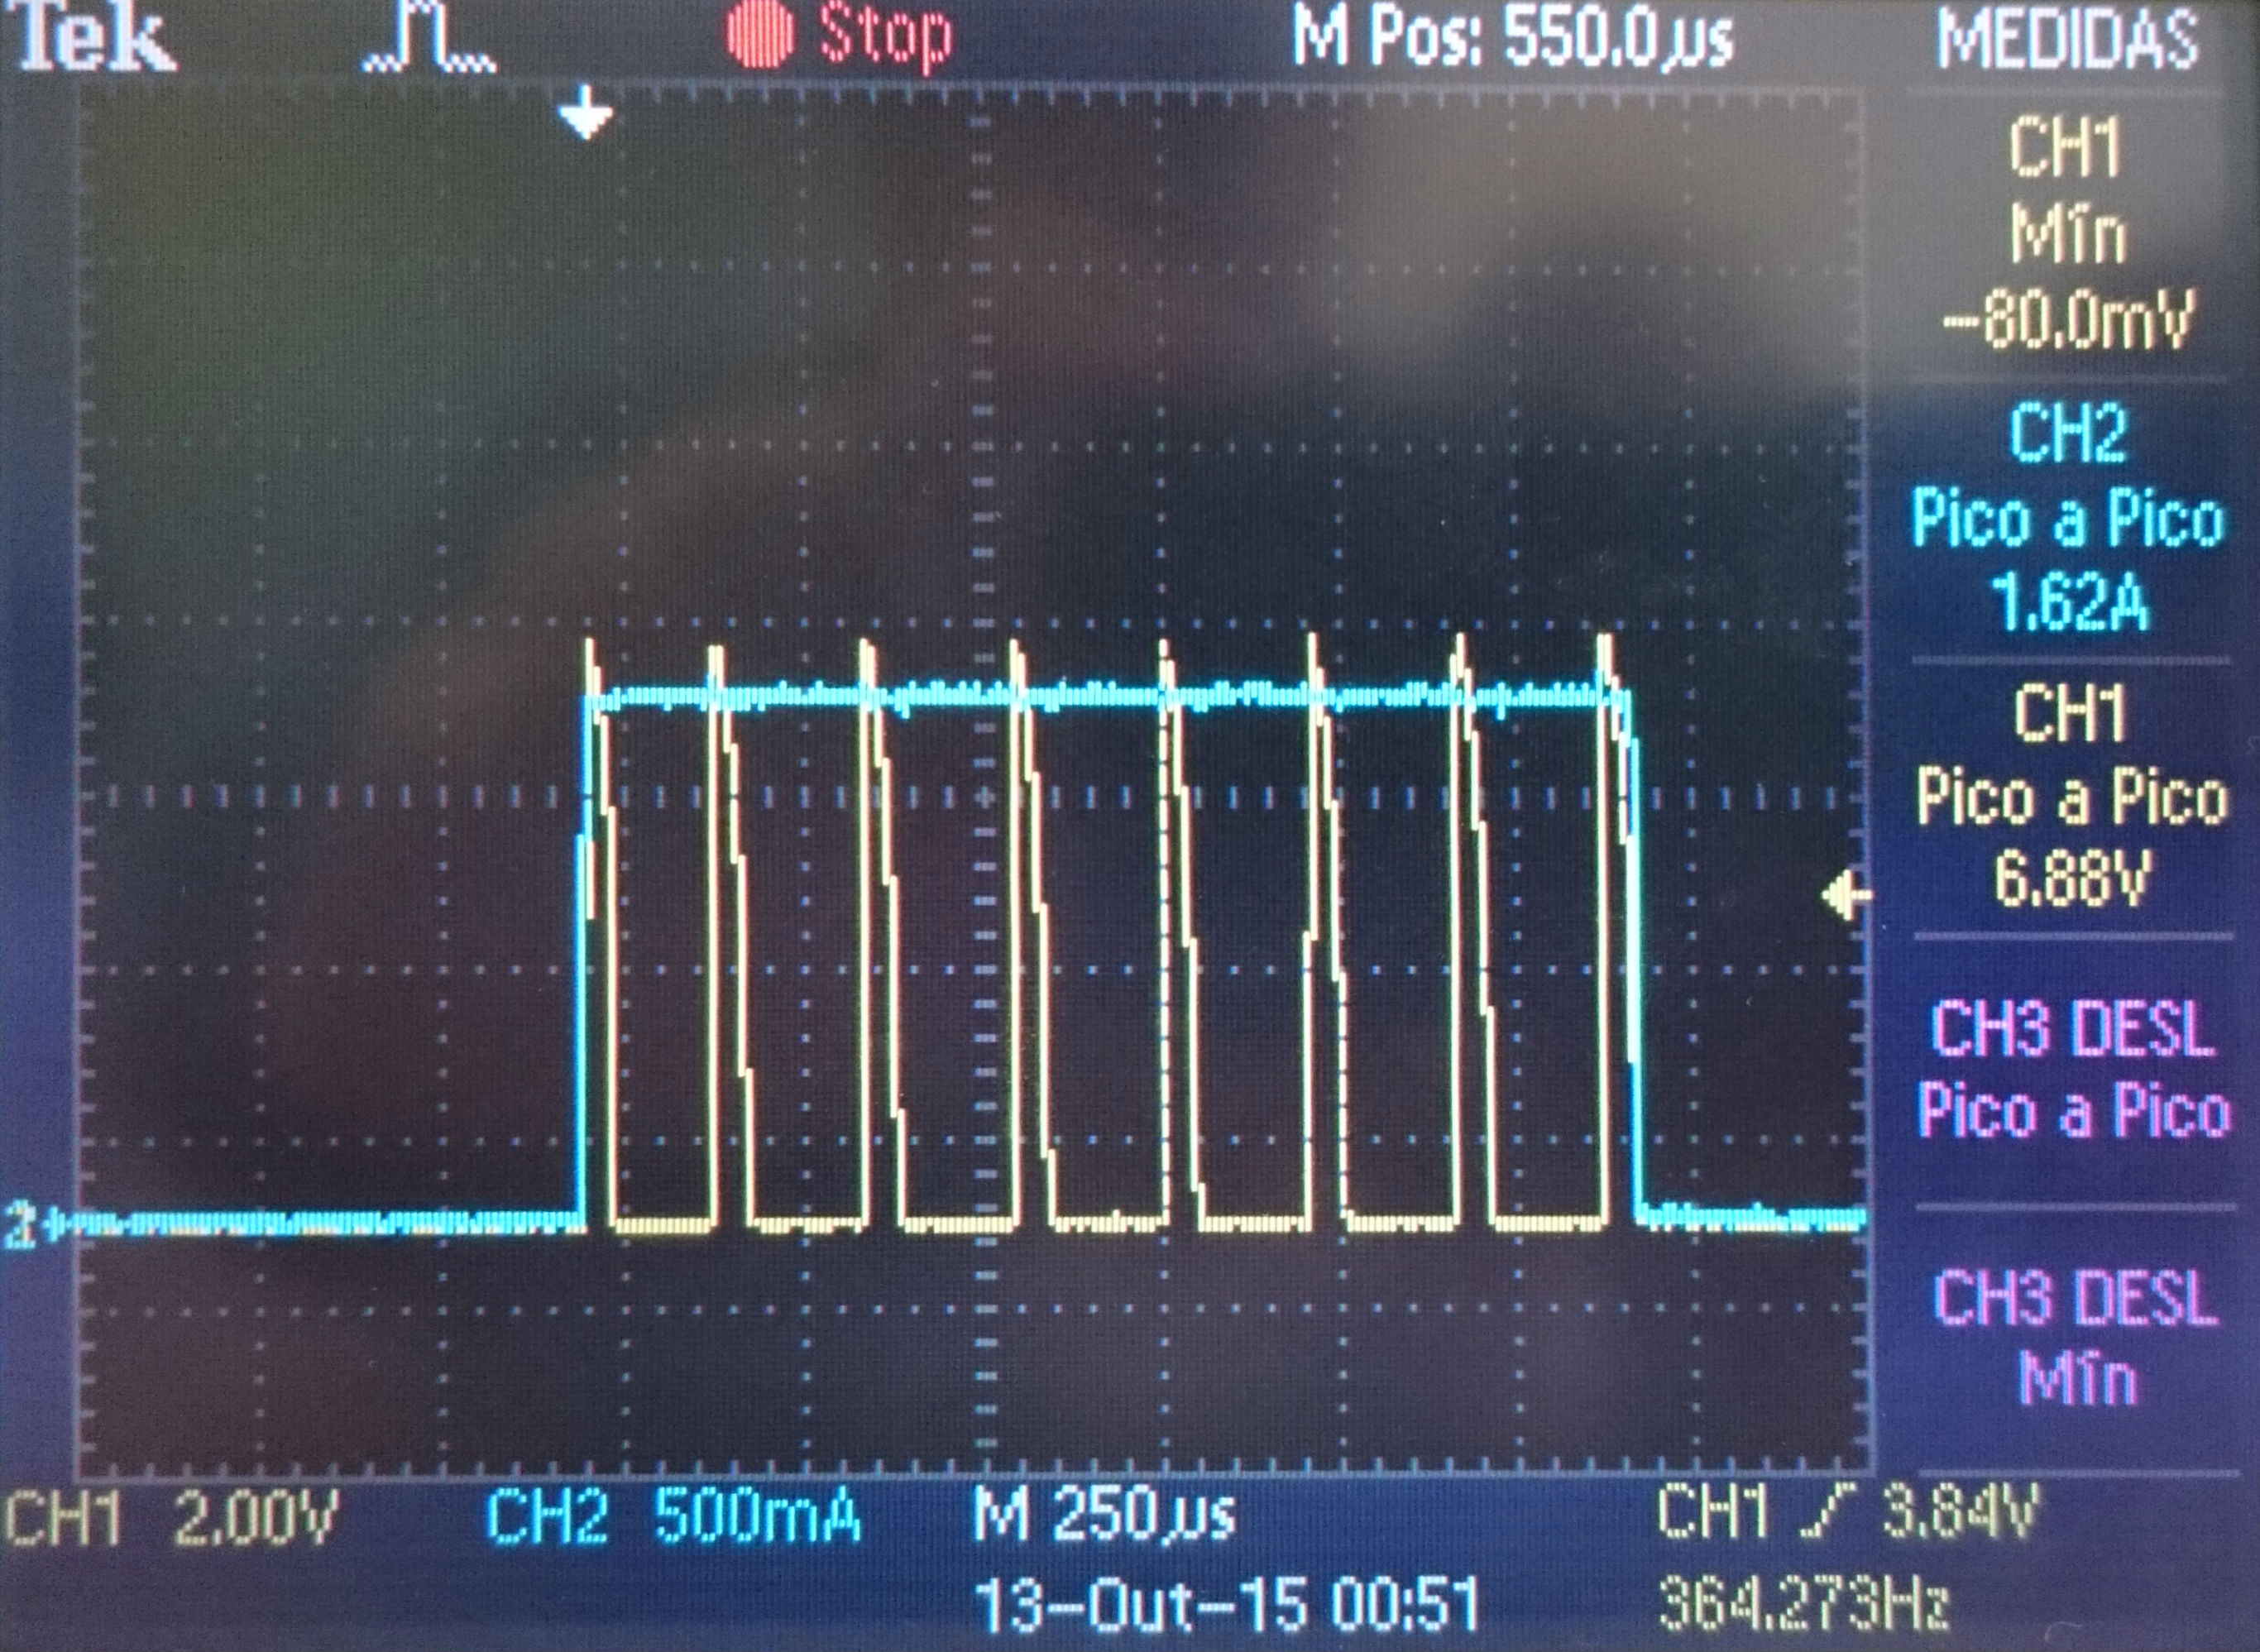
\includegraphics[keepaspectratio=true, scale=0.09]{img/figs/trem_impulsos_B}
	\caption{Formas de onda do trem de impulso e tensão em B.}
	\label{fig:trem_impulsos_B}
	\vspace{-0.8em}
\end{figure}

Na \autoref{fig:trem_impulsos_B} pode também observar-se o trem de impulsos, a amarelo, face ao impulso original correspondente, a azul.


\subsection{Estudo do circuito de potência}

\subsubsection{Carga resistiva pura (R)}

Para que se possa estudar o funcionamento do retificador para cargas do tipo resistivas puras utilizou-se um reóstato como carga, regulando-o para uma carga de aproximadamente $16$ $\Omega$.

\paragraph{Formas de onda da tensão e corrente na entrada e na carga}\mbox{}\

\begin{figure}[H]
	\centering
	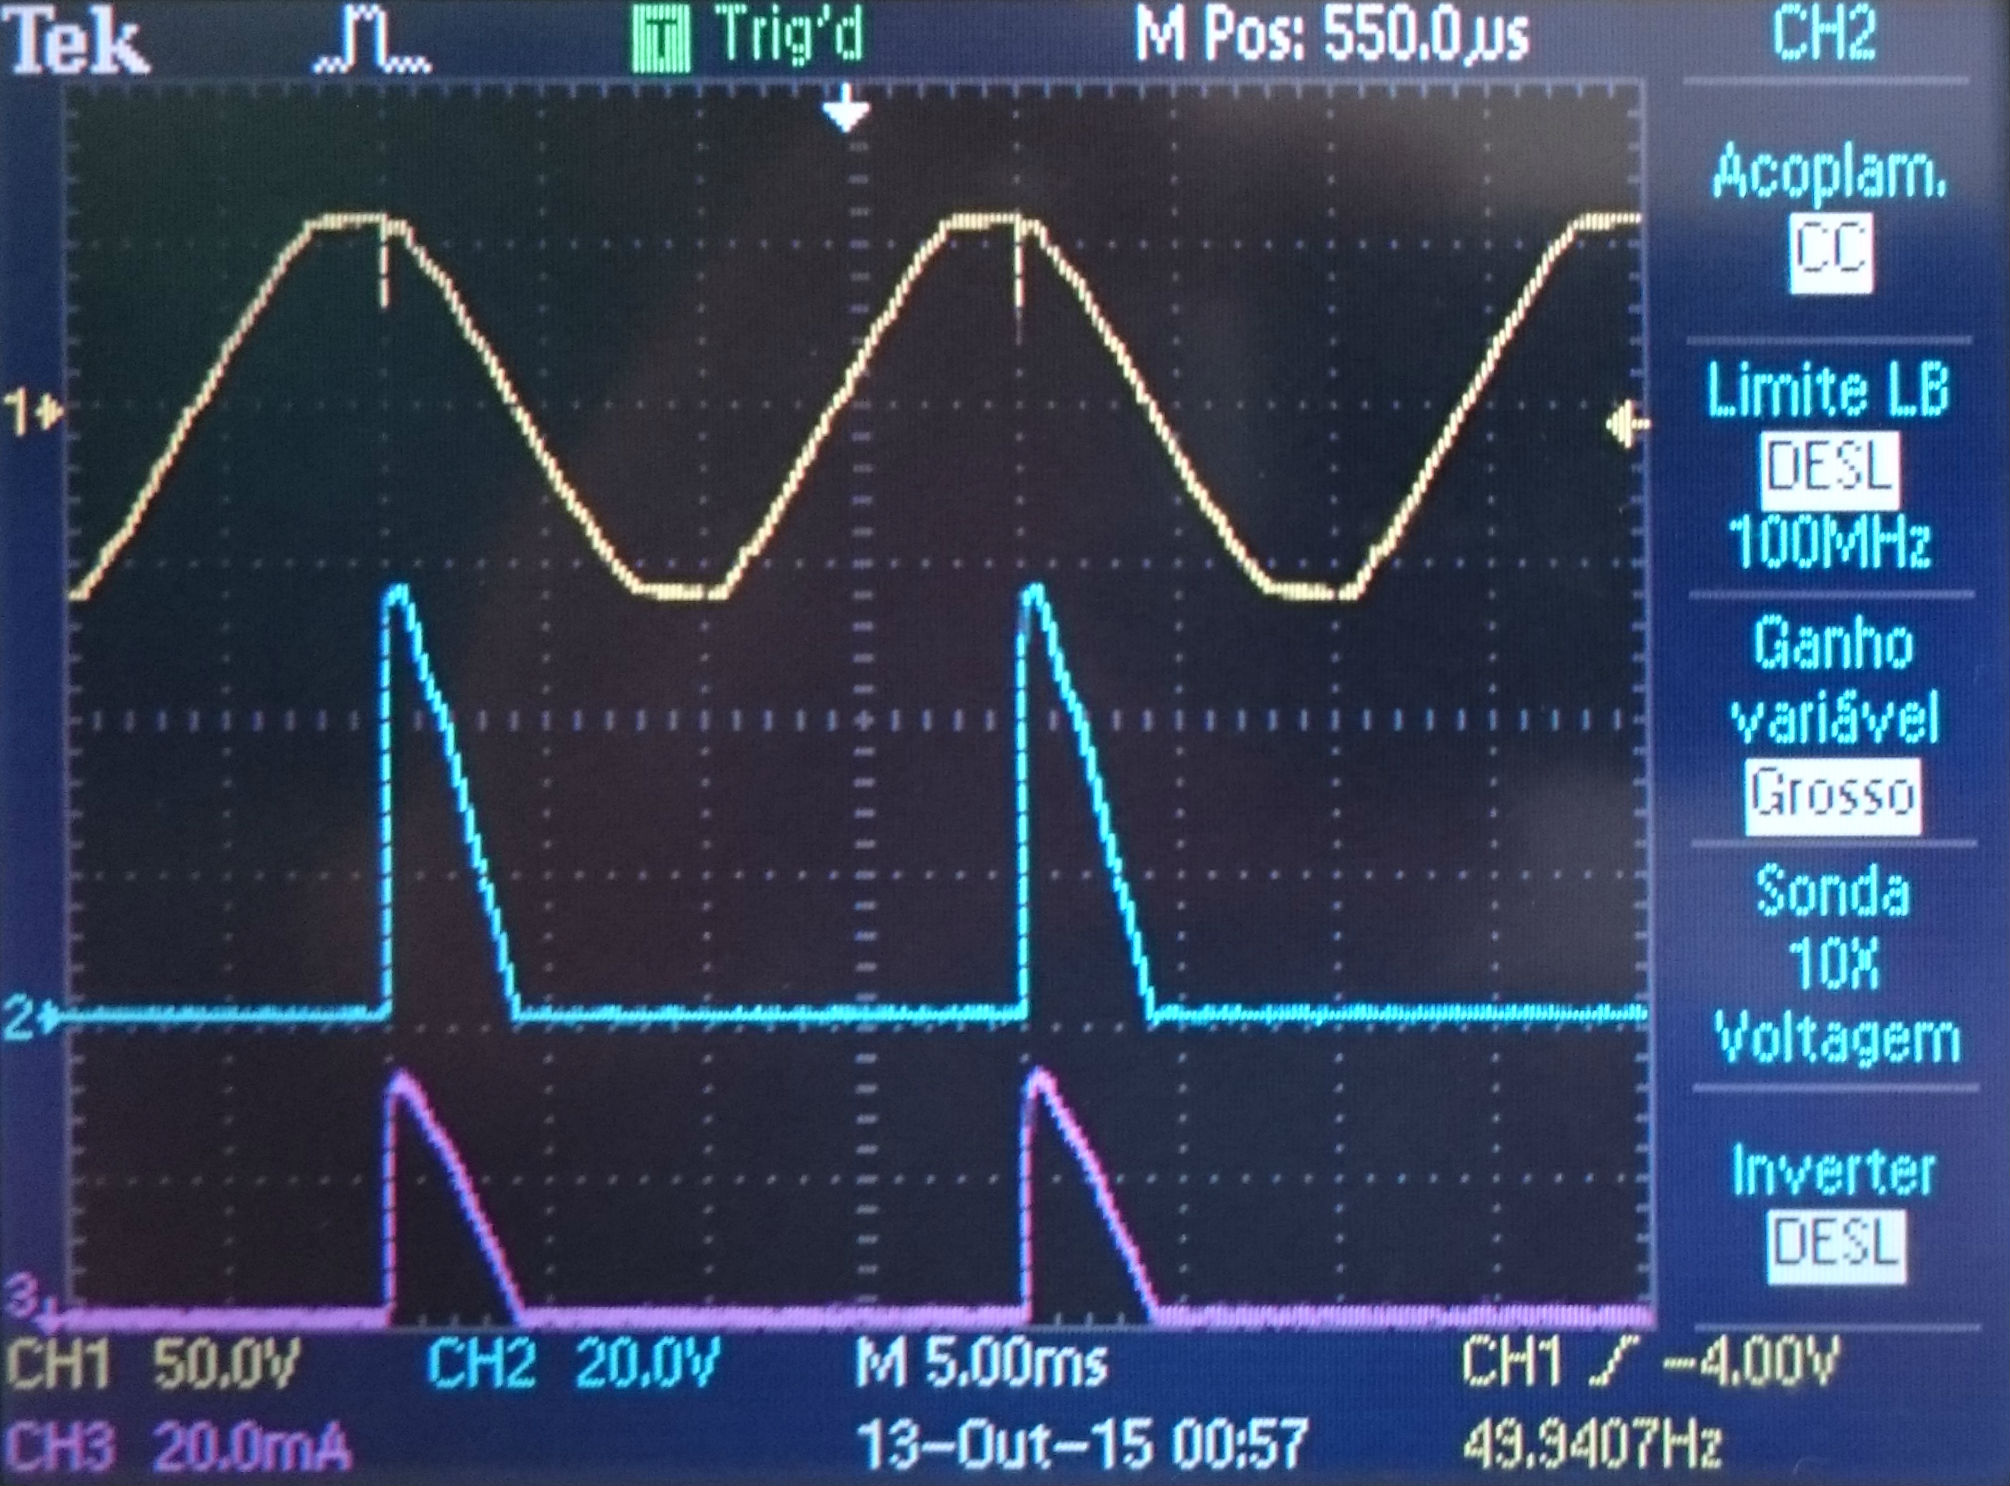
\includegraphics[keepaspectratio=true, scale=0.12]{img/figs/carga_resistiva}
	\caption{Formas da tensão na entrada e corrente e tensão na carga para carga R.}
	\label{fig:carga_resistiva}
	\vspace{-0.8em}
\end{figure}


Na \autoref{fig:carga_resistiva} observa-se o funcionamento do circuito quando sujeito uma carga resistiva pura. A tensão de entrada pode ser vista a amarelo estando a tensão e corrente na carga a azul e roxo respetivamente.

%\paragraph{Formas de onda da tensão e corrente na saída}\mbox{}\


%\unsure{pode apagar-se esta secção porque a imagem ja foi mostrada na anterior}

\paragraph{Formas de onda da tensão e corrente no tiristor}\mbox{}\

\unsure{não temos esta imagem. Podemos roubar a imagem do edson ou ser honestos, dizer que nos esquecemos de tirar a foto e por aqui uma imagem da simualação equivalente}

\paragraph{Valores médio e eficaz da tensão e corrente na carga}\mbox{}\

Os valores médio e eficaz de tensão e corrente na carga podem ser obtidos através das seguintes expressões:


\begin{equation}
v_i(t)=A \sin(\omega t)
\end{equation}

\begin{equation}
V_{o_{MED}} (t) = \frac{1}{2\pi} \int_{\alpha}^{\pi} A \sin(\omega t) d \omega t = \frac{A}{2\pi} (1+ \cos\alpha)
\end{equation}

\begin{equation}
I_{o_{MED}}= \frac{V_{o_{MED}}}{R}
\end{equation}

\begin{equation}
V_{o_{RMS}} = \sqrt{ \frac{1}{2\pi} \int_{\alpha}^{\pi} A^2 \sin^2 (\omega t) d\omega t} = \sqrt{ \frac{A^2}{8 \pi} (2\pi - 2\alpha + \sin(2\alpha))}
\end{equation}

\begin{equation}
I_{o_{RMS}}= \frac{V_{o_{RMS}}}{R}
\end{equation}


Infelizmente não se mediu os valores necessários no laboratório pelo que estes serão assumidos de forma a exemplificar como seria feito o cálculo teórico.

Por observação da \autoref{fig:carga_resistiva} tem-se $A=52$ V e $\alpha=0,55\pi$ rad. Assume-se também que a resistência na carga toma o valor $R=15~\Omega$.

Os valores obtidos teoricamente são:

\[V_{o_{MED}} (t) = \frac{52}{2\pi} \left(1+ \cos0,55\pi \right) = 6,98~\text{V}\]

\[I_{o_{MED}}= \frac{6,98}{15} = 465~\text{mA}\]

\[V_{o_{RMS}} = \sqrt{ \frac{52^2}{8 \pi} \left(2\pi - 2\left(0,55\pi\right) + \sin\left(2(0,55\pi\right)\right)} = 20,26~\text{V} \]

\[I_{o_{RMS}}= \frac{20,26}{15} = 1,35~\text{A}\]

Tal como foi mencionado, não foram registados os valores laboratoriais, no entanto, pode-se fazer uma estimativa grosseira dos valores médios de corrente e tensão na carga, considerando que durante três quartos do período ambas as grandezas estão a zero, que a forma da onda é perfeitamente triangular e que existe uma atenuação de 100 vezes na sonda de corrente.

\[V_{o_{MED}} (t) = \frac{\frac{48}{2}}{4} = 6~\text{V}\]

\[I_{o_{MED}}= \frac{\frac{0,036}{2}}{4} = 450~\text{mA}\]

\vspace{3mm}

Sendo assim, considerando que o valor de $R$ considerado poderá ser diferente do utilizado no laboratório, cujo máximo seria perto de $100~\Omega$, pode considerar-se que os valores teóricos serão próximos dos reais, fora algumas incertezas.

\paragraph{Característica de comando do conversor}\mbox{}\

Para se estudar convenientemente o funcionamento do circuito face a variações do ângulo de disparo $\alpha$, registaram-se os valores da tensão na carga em função deste tanto no caso experimental como teórico fazendo uso das expressões da secção anterior. Os resultados obtidos podem ser observados na \autoref{tab:tabela1} e \autoref{fig:grafico1}. 

\begin{table}[!htb]
	\centering
	\caption{Valores da tensão na carga, teóricos e experimentais, em função de $\alpha$.}
	\vspace{-3mm}
	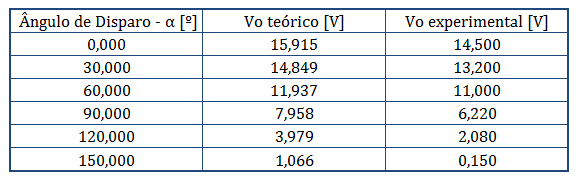
\includegraphics[width=0.8\linewidth]{teoricas/tabela1}
	\label{tab:tabela1}
\end{table}

\begin{figure}[H]
	\centering
	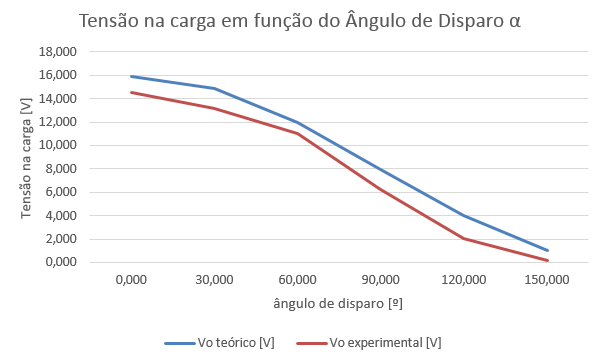
\includegraphics[keepaspectratio=true, scale=0.8]{teoricas/grafico1}
	\vspace{-3mm}
	\caption{Formas de onda da tensão na carga, teóricas e experimentais, em função de $\alpha$.}
	\label{fig:grafico1}
	\vspace{-0.8em}
\end{figure}

\todo{falta por a lengeda nos eixos do grafico e as unidades}

Verifica-se que existe pouca diferença entre os valores, podendo estas dever-se maioritariamente com o facto de, para os cálculos teóricos, se considerar que todos os dispositivos são ideais, o que não é válido na realidade.

\subsubsection{Carga indutiva RL}

Para estudar o comportamento de um retificador de meia onda com uma carga indutiva introduziu-se uma bobina em série com o reóstato.

\paragraph{Formas de onda da tensão e corrente na saída}\mbox{}\

\begin{figure}[h]
	\centering
	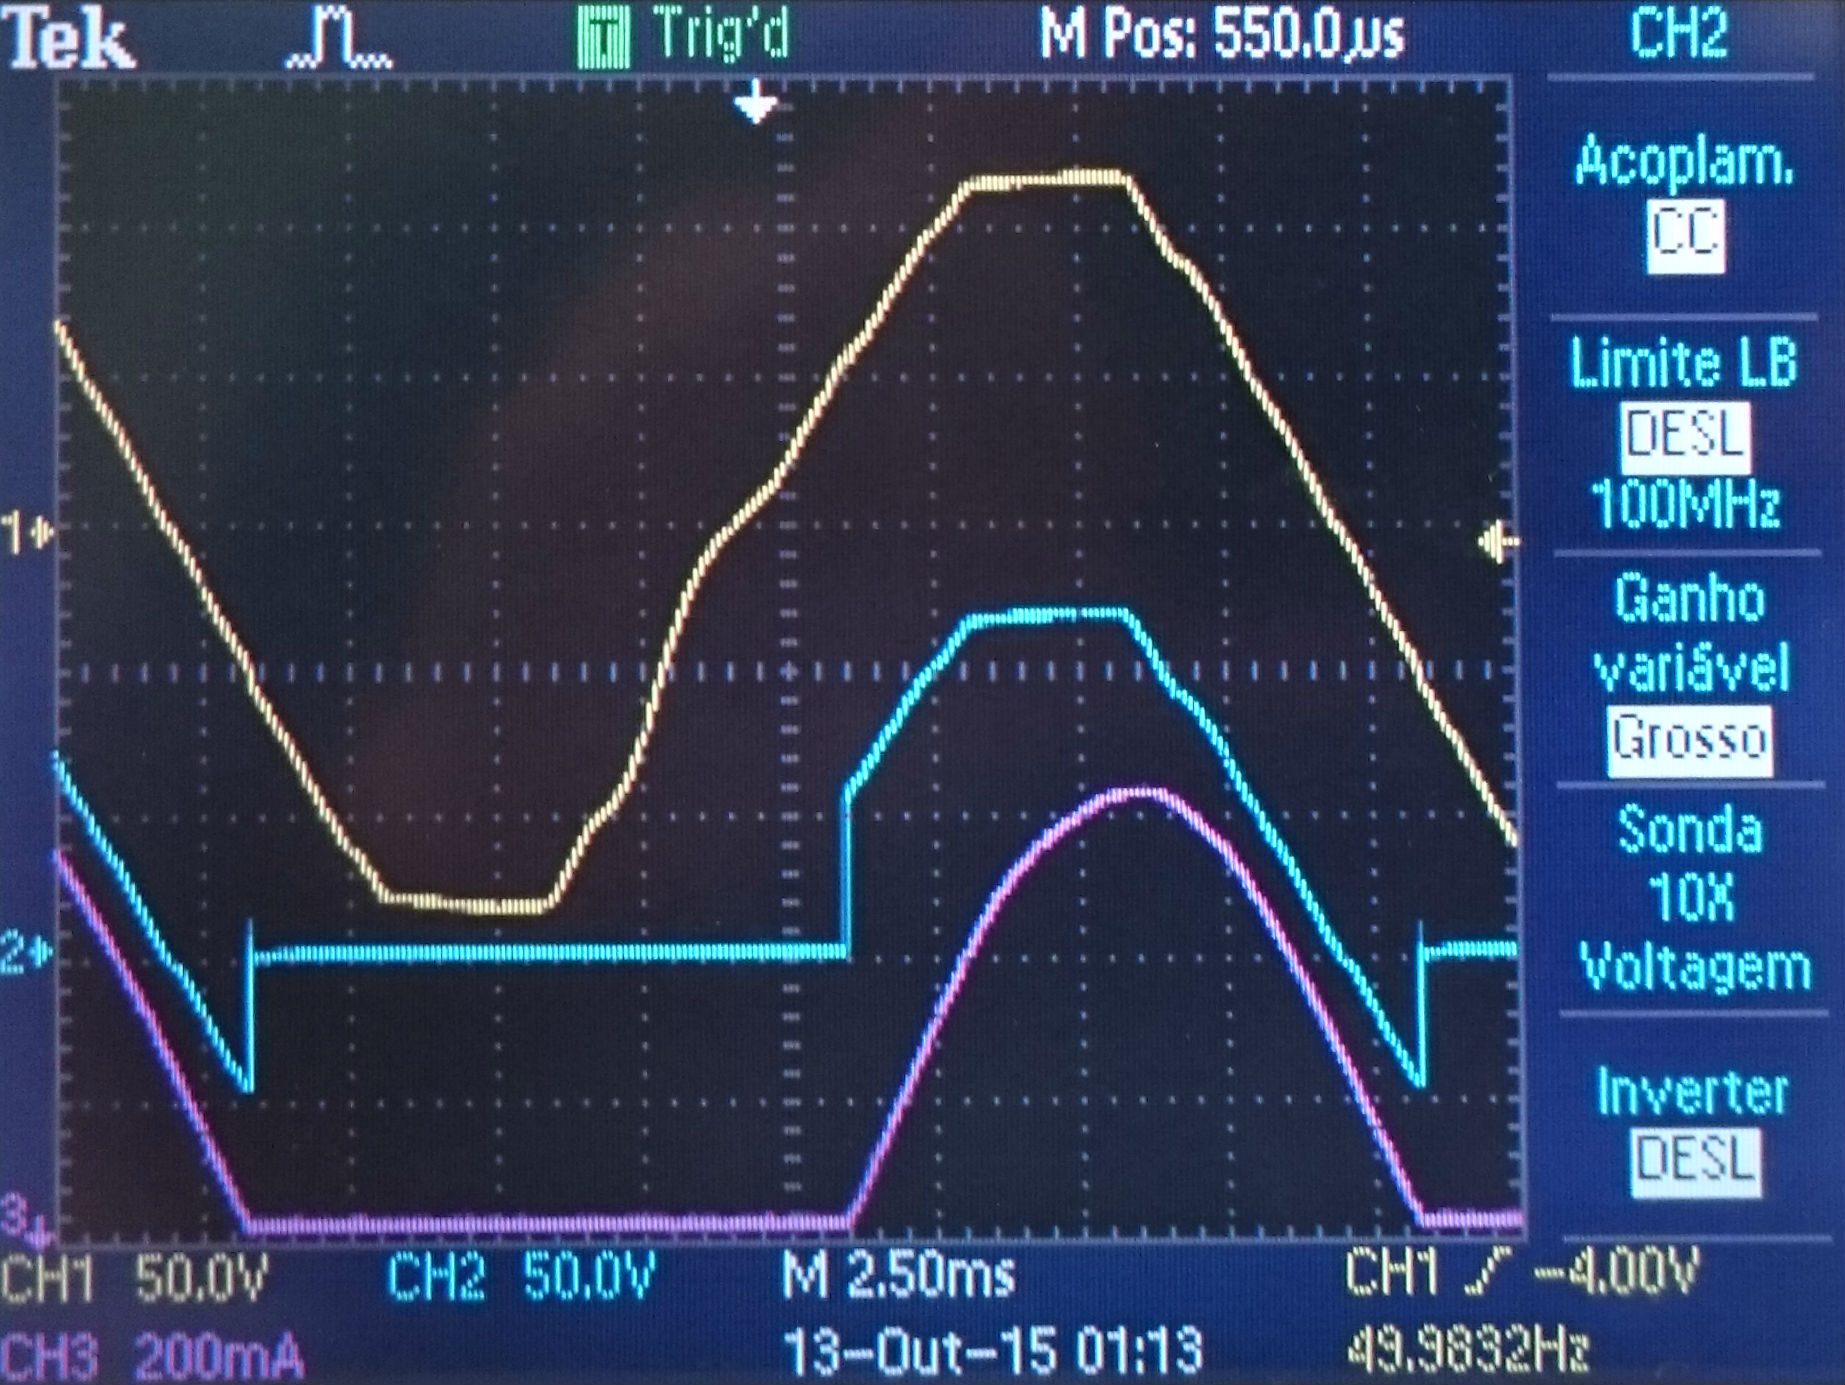
\includegraphics[keepaspectratio=true, scale=0.13]{img/figs/carga_indutiva}
	\caption{Formas de onda de tensão na entrada e tensão e corrente na saída para carga indutiva.}
	\label{fig:carga_indutiva}
	\vspace{-0.8em}
\end{figure}

Na \autoref{fig:carga_indutiva} podem ser observadas as formas de onda da tensão (a amarelo) na entrada do retificador e a tensão (a azul) e corrente (a rosa) na carga.

\paragraph{Formas de onda da tensão e corrente no tiristor}\mbox{}\

A tensão no tiristor $V_{AK}$ é $0$ quando o dispositivo está a conduzir, e é igual à tensão de entrada quando o dispositivo está ao corte, isto é, $V_{AK} = V_I - V_O$.

Uma vez que o tiristor se encontra em série com a carga (trata-se de um rectificador de meia onda), a corrente no tiristor é idêntica à corrente da carga.

Assim, a forma de onda da corrente no tiristor corresponde à corrente da \autoref{fig:carga_indutiva}, e a tensão no dispositivo corresponde à forma de onda complementar à tensão da mesma figura.

\paragraph{Análise teórica do circuito}\mbox{}\

\todo{rever esta parte}

A montagem pode ser simplificada para o circuito da \autoref{fig:ci_circuito}, considerando a saída do transformador como uma fonte de tensão alternada.

\begin{figure}[h]
	\centering
	\begin{tikzpicture}
		\draw
		(0,0) node[] (sourcetop) {}
		(0,-2) node[] (sourcebottom) {}		
		
		(sourcetop) to[sV,v=$ $] (sourcebottom)
		
		(sourcetop) to[Ty, n=thyr] ++(3,0) to[L, l=$10 mH$] ++ (3,0) to[R,l=$15 \Omega$]++(0,-2) to[short] (sourcebottom)
		;
	\end{tikzpicture}
	\caption{Circuito em análise com carga indutiva}
	\label{fig:ci_circuito}
\end{figure}

A partir de $\omega t = \alpha$, enquanto o tiristor está a conduzir, o comportamento do circuito é dado pela \autoref{eq:ci_eqdif}.

\begin{equation}
\label{eq:ci_eqdif}
v_O = R\,i_{O} + L \frac{\mathrm{d}}{\mathrm{d}t}i_O
\end{equation}

A \autoref{eq:ci_eqdif} resulta nas \autoref{eq:ci_eqs}.

\begin{subequations}
\label{eq:ci_eqs}
\begin{align}
i_{O\;\text{livre}} &= A\,e^{-\frac{R}{L}(t - \frac{\alpha}{\omega})}\\
i_{O\;\text{forçado}} &= \sqrt{2} \frac{V}{Z} \sin{(\omega t - \Phi)}\\
i_O &= i_{O\;\text{livre}} + i_{O\;\text{forçado}}
\end{align}
\end{subequations}

Quando a tensão de entrada passa à arcada negativa, o tiristor não pode passar ao corte, uma vez que a corrente na bobina é uma variável de estado e não se pode anular.

Quando a corrente na bobina finalmente se anula ($\omega t = \beta$), o tiristor passa ao corte.

Ao contrário do que se tinha no caso da carga resistiva, a tensão na carga irá consequentemente apresentar valores negativos.


\subsubsection{Carga indutiva RL e díodo de roda livre}

Por fim, introduz-se no retificador um díodo de roda livre em antiparalelo com a carga para se estudar o seu impacto no circuito.

Teoricamente a introdução deste díodo deverá garantir que a tensão na carga não passará de zero devido à adição de uma indutância, pelas razões comentadas anteriormente.


\paragraph{Formas de onda da tensão e corrente na saída \label{parag:1}}\mbox{}\

\begin{figure}[h]
	\centering
	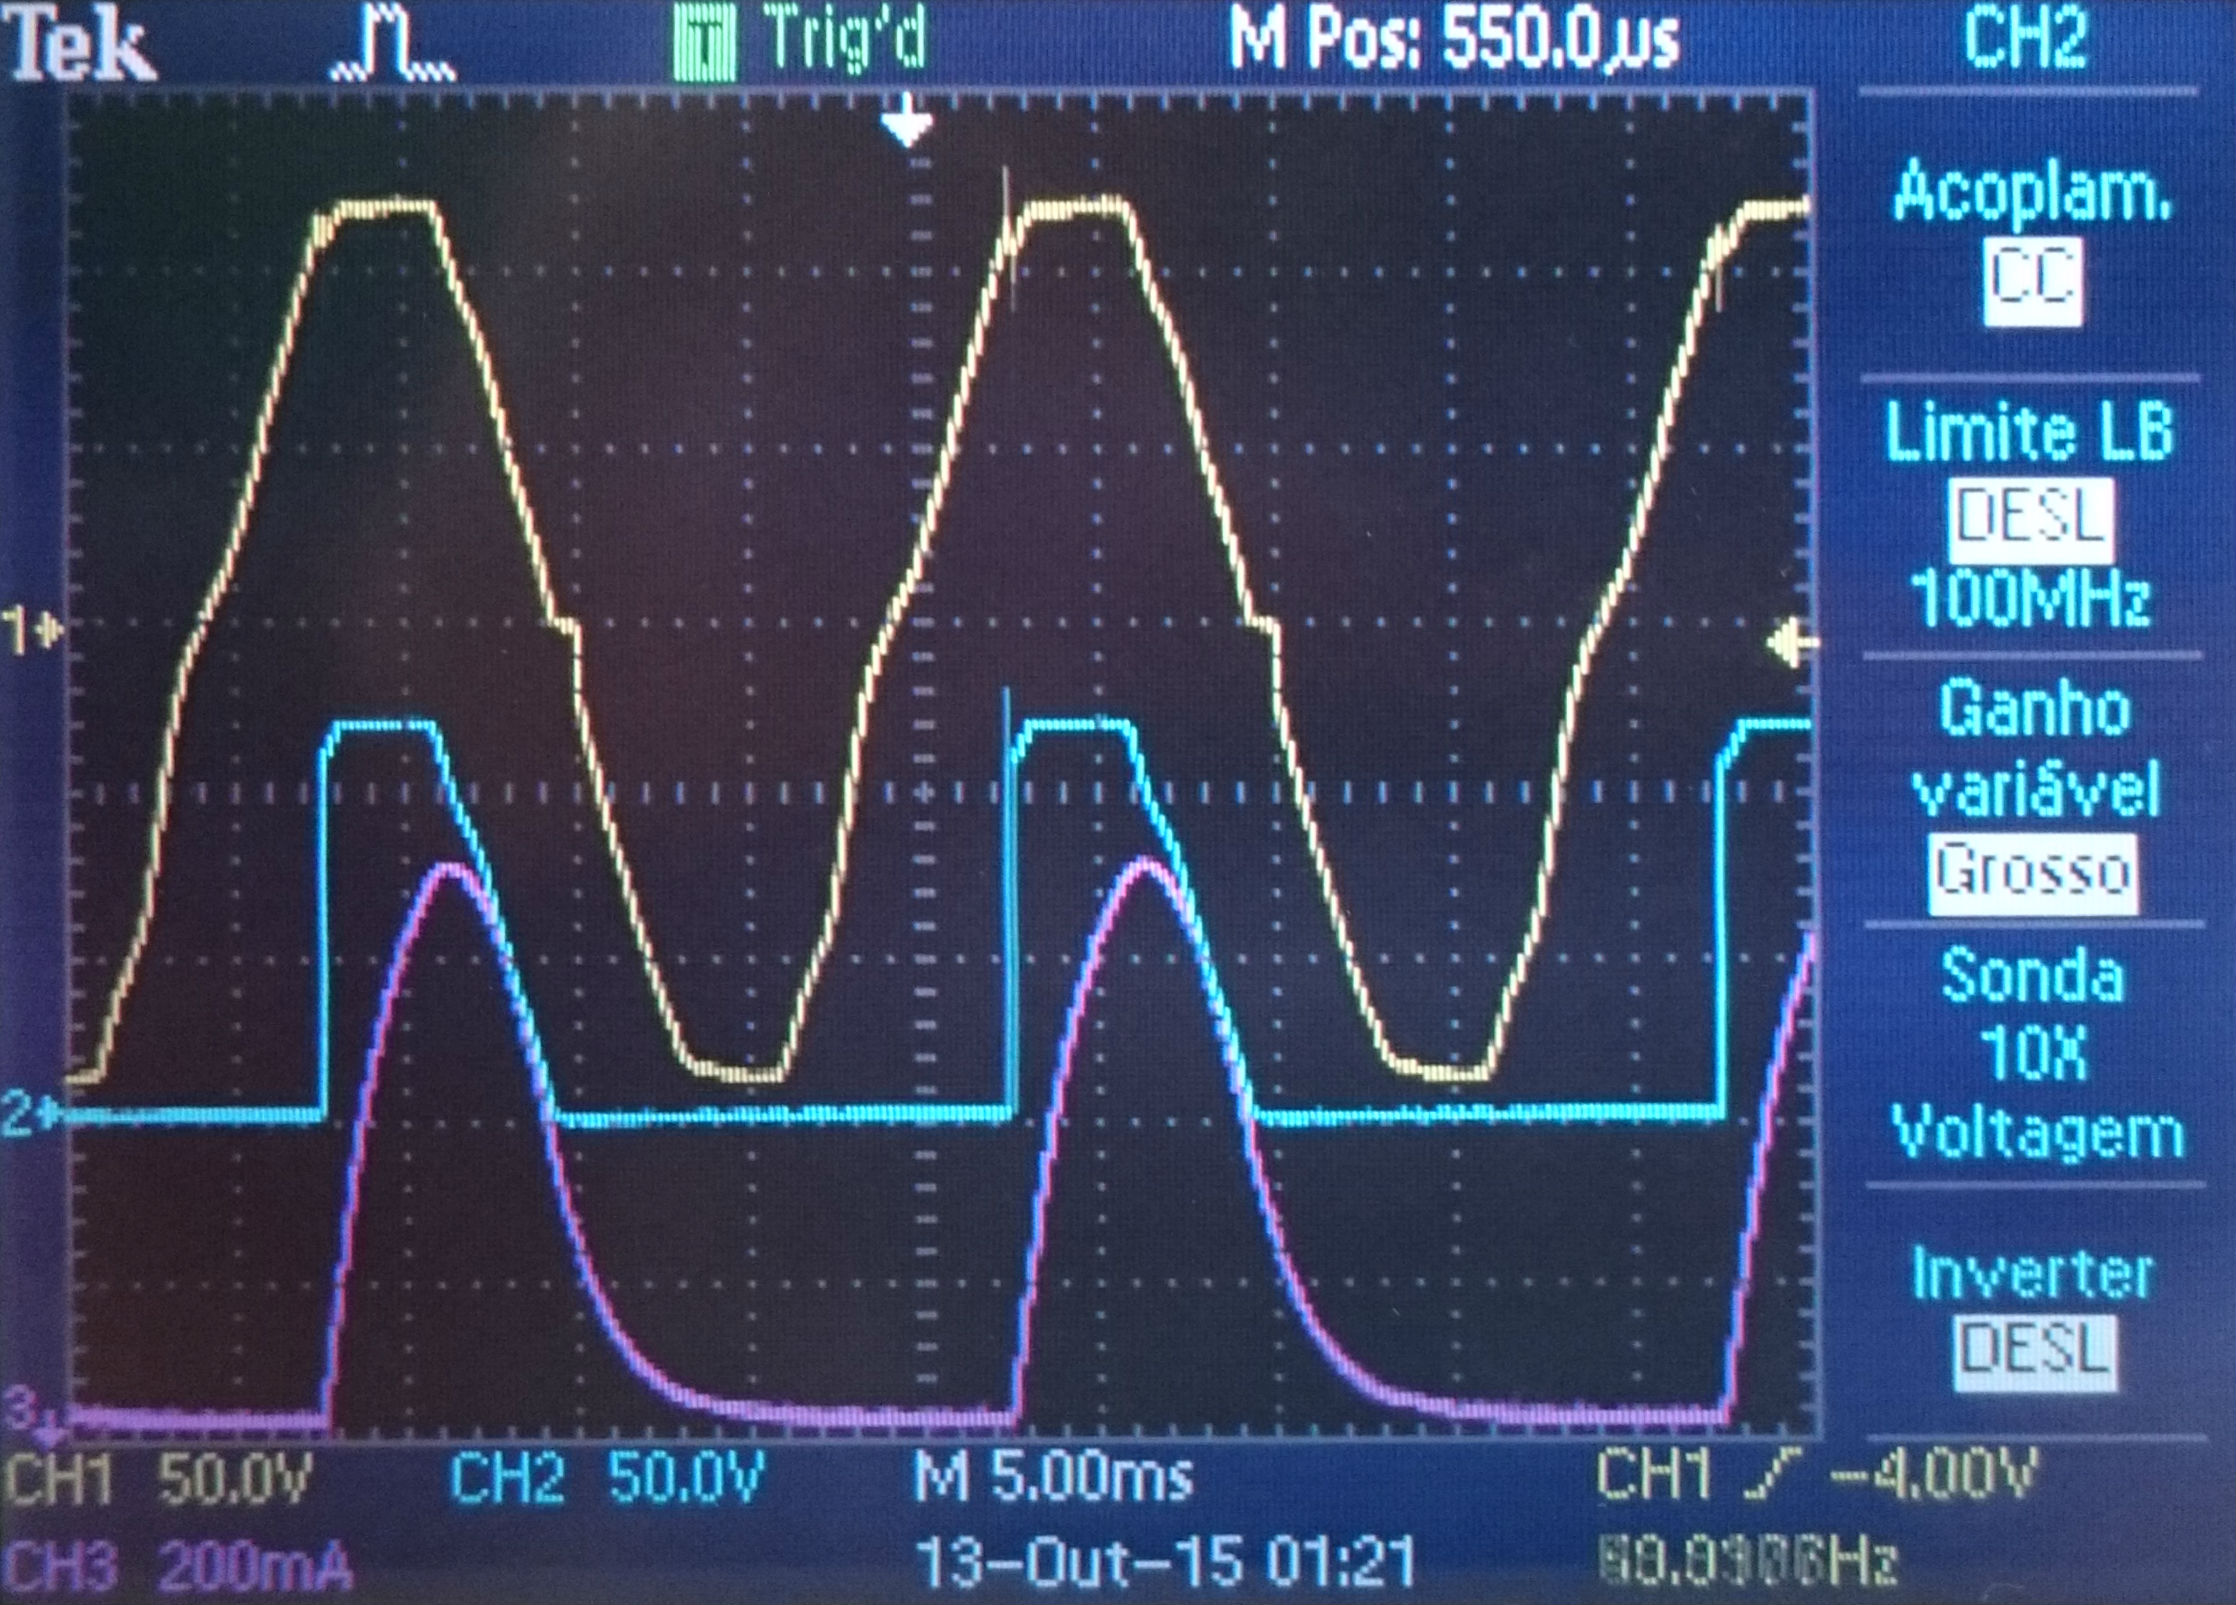
\includegraphics[keepaspectratio=true, scale=0.11]{img/figs/bobine_alfa_dif_zero}
	\caption{Formas de onda da tensão na entrada e tensão e corrente na saída para carga indutiva com $\alpha$ diferente de zero.}
	\label{fig:bobine_alfa_dif_zero}
	\vspace{-0.8em}
\end{figure}

Na \autoref{fig:bobine_alfa_dif_zero} tem-se a tensão na entrada do retificador (a amarelo) e tensão (a azul) e corrente (a rosa) na carga.

Observa-se que existe um ligeiro intervalo no qual a tensão na carga ainda é menor que zero, embora um valor muito inferior ao que se tinha no caso da carga RL sem díodo de roda livre. Isto deve-se a que nesse período a tensão observável será igual à de polarização direta do díodo de roda livre, que como está em antiparalelo com a carga, entra em condução na alternância negativa da tensão. 

\paragraph{Formas de onda da tensão e corrente no tiristor}\mbox{}\

\begin{figure}[H]
	\centering
	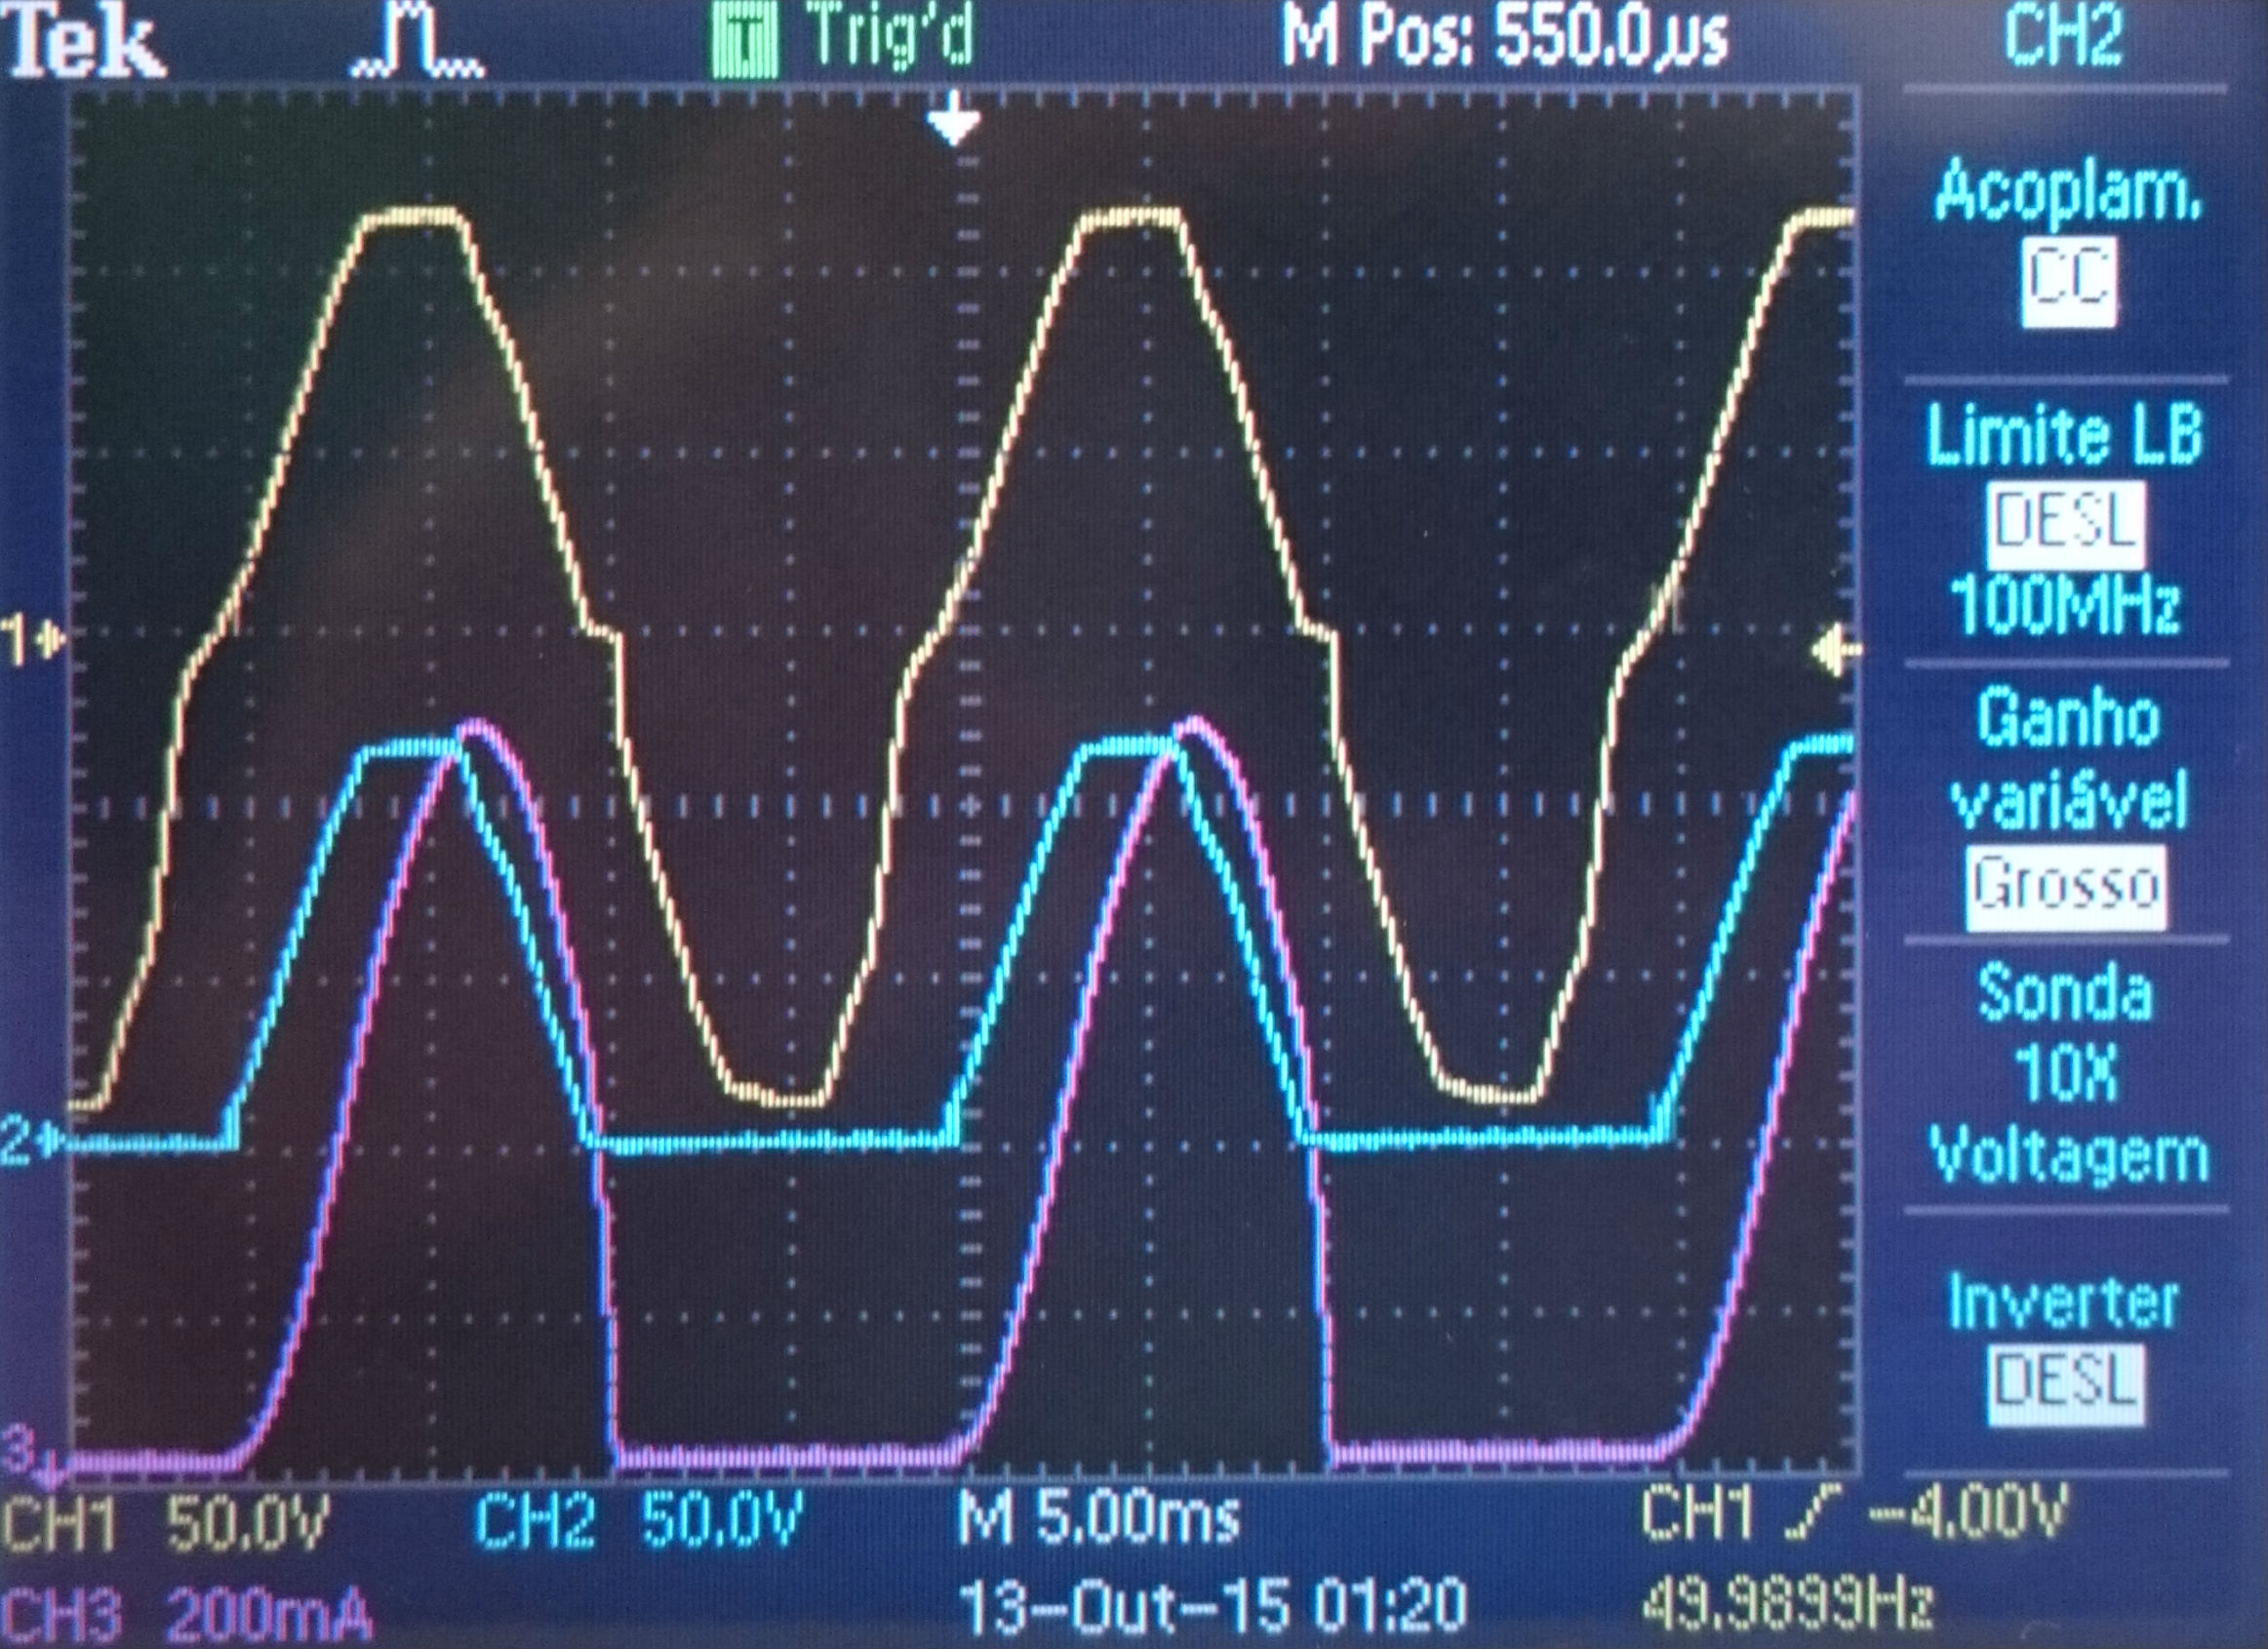
\includegraphics[keepaspectratio=true, scale=0.11]{img/figs/tiristor_alfa_zero}
	\caption{Formas de onda da tensão na entrada e corrente no tiristor para carga indutiva.}
	\label{fig:tiristor_alfa_zero}
	\vspace{-0.8em}
\end{figure}

\begin{figure}[H]
	\centering
	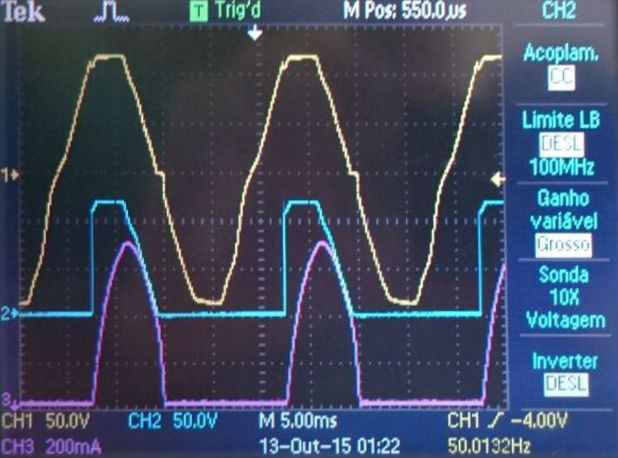
\includegraphics[keepaspectratio=true, scale=0.43]{img/figs/tiristor_alfa_dif_zero}
	\caption{Formas de onda de tensão na entrada e corrente no tiristor para carga indutiva com $\alpha$ diferente de zero.}
	\label{fig:tiristor_alfa_dif_zero}
	\vspace{-0.8em}
\end{figure}

Na \autoref{fig:tiristor_alfa_zero} tem-se a tensão na entrada do retificador (a amarelo) e corrente (a rosa) no tiristor, para $\alpha = 0$, sendo o comportamento para $\alpha$ diferente de $0$ observável na \autoref{fig:tiristor_alfa_dif_zero}.

Nestas figuras no entanto não se observa a tensão aos terminais do tiristor (a azul tem-se sim a tensão na carga). O comportamento expectável para esta seria apresentar o valor de tensão de polarização direta enquanto o dispositivo está à condução e a tensão na entrada do retificador enquanto está ao corte.

\paragraph{Formas de onda da tensão e corrente no díodo e na bobina}\mbox{}\

\begin{figure}[H]
	\centering
	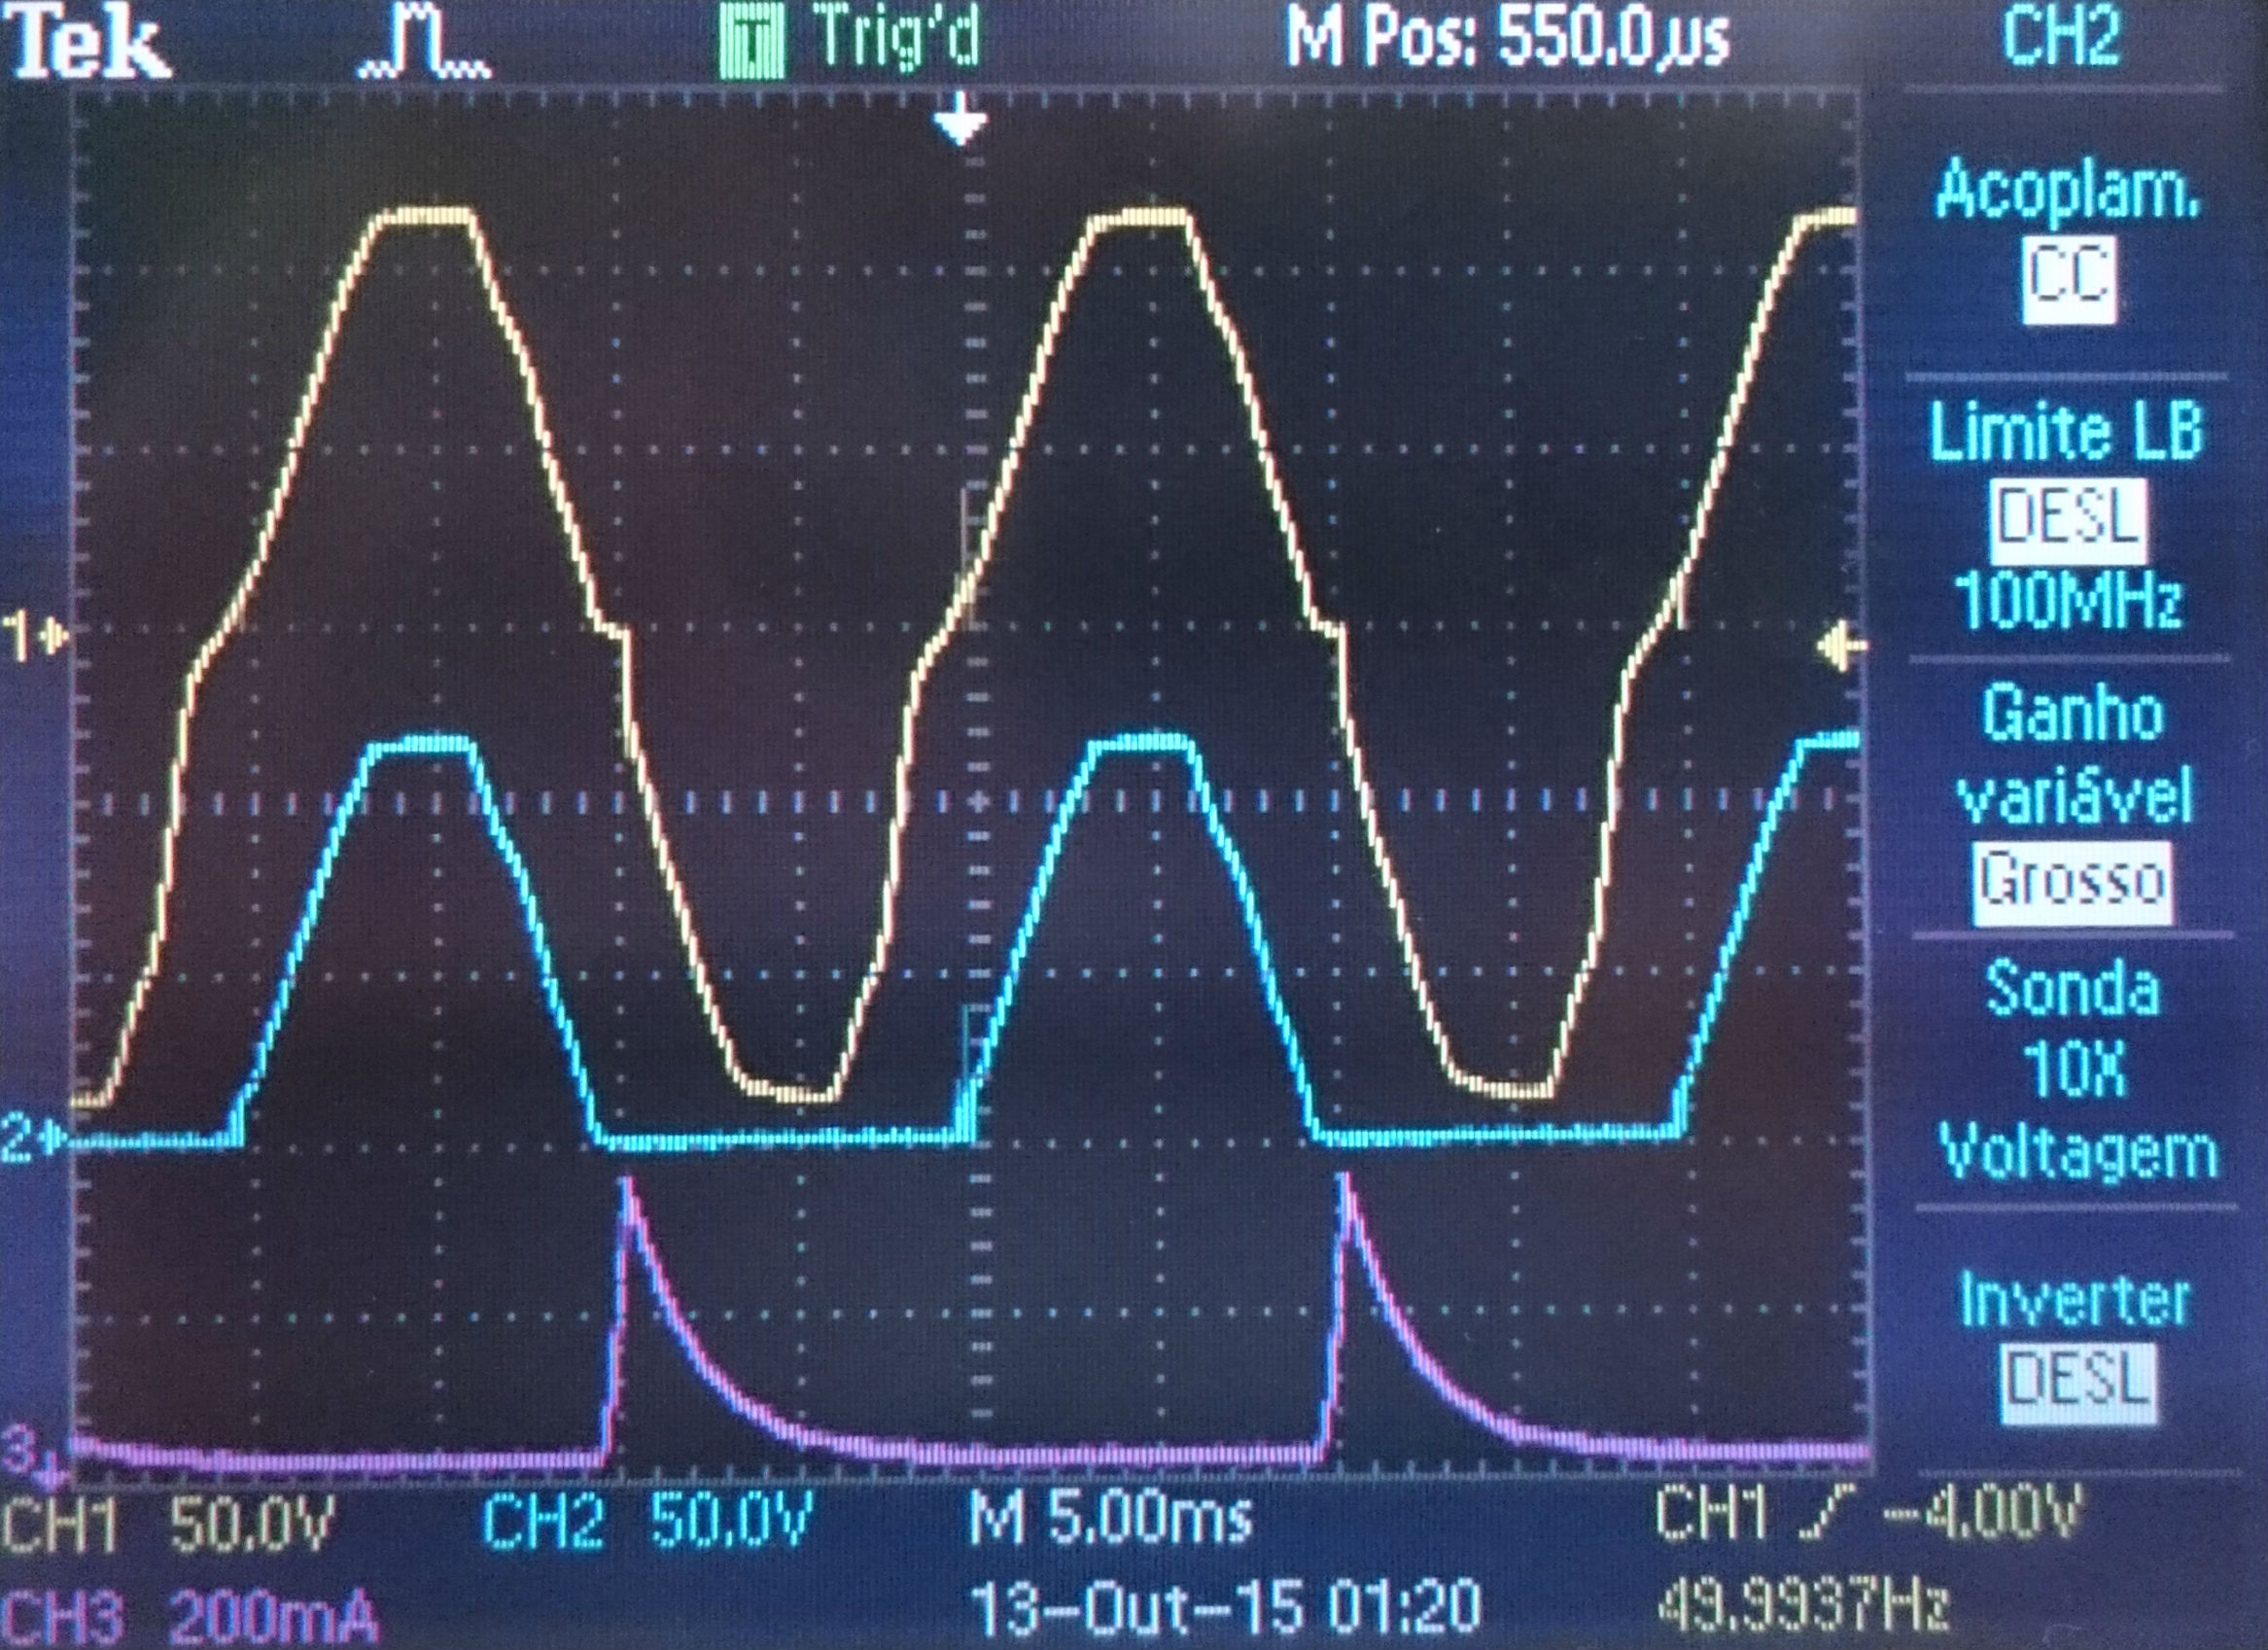
\includegraphics[keepaspectratio=true, scale=0.12]{img/figs/diodo_alfa_zero}
	\caption{Formas de onda da tensão na entrada e corrente no diodo para carga indutiva.}
	\label{fig:diodo_alfa_zero}
	\vspace{-0.8em}
\end{figure}

\begin{figure}[H]
	\centering
	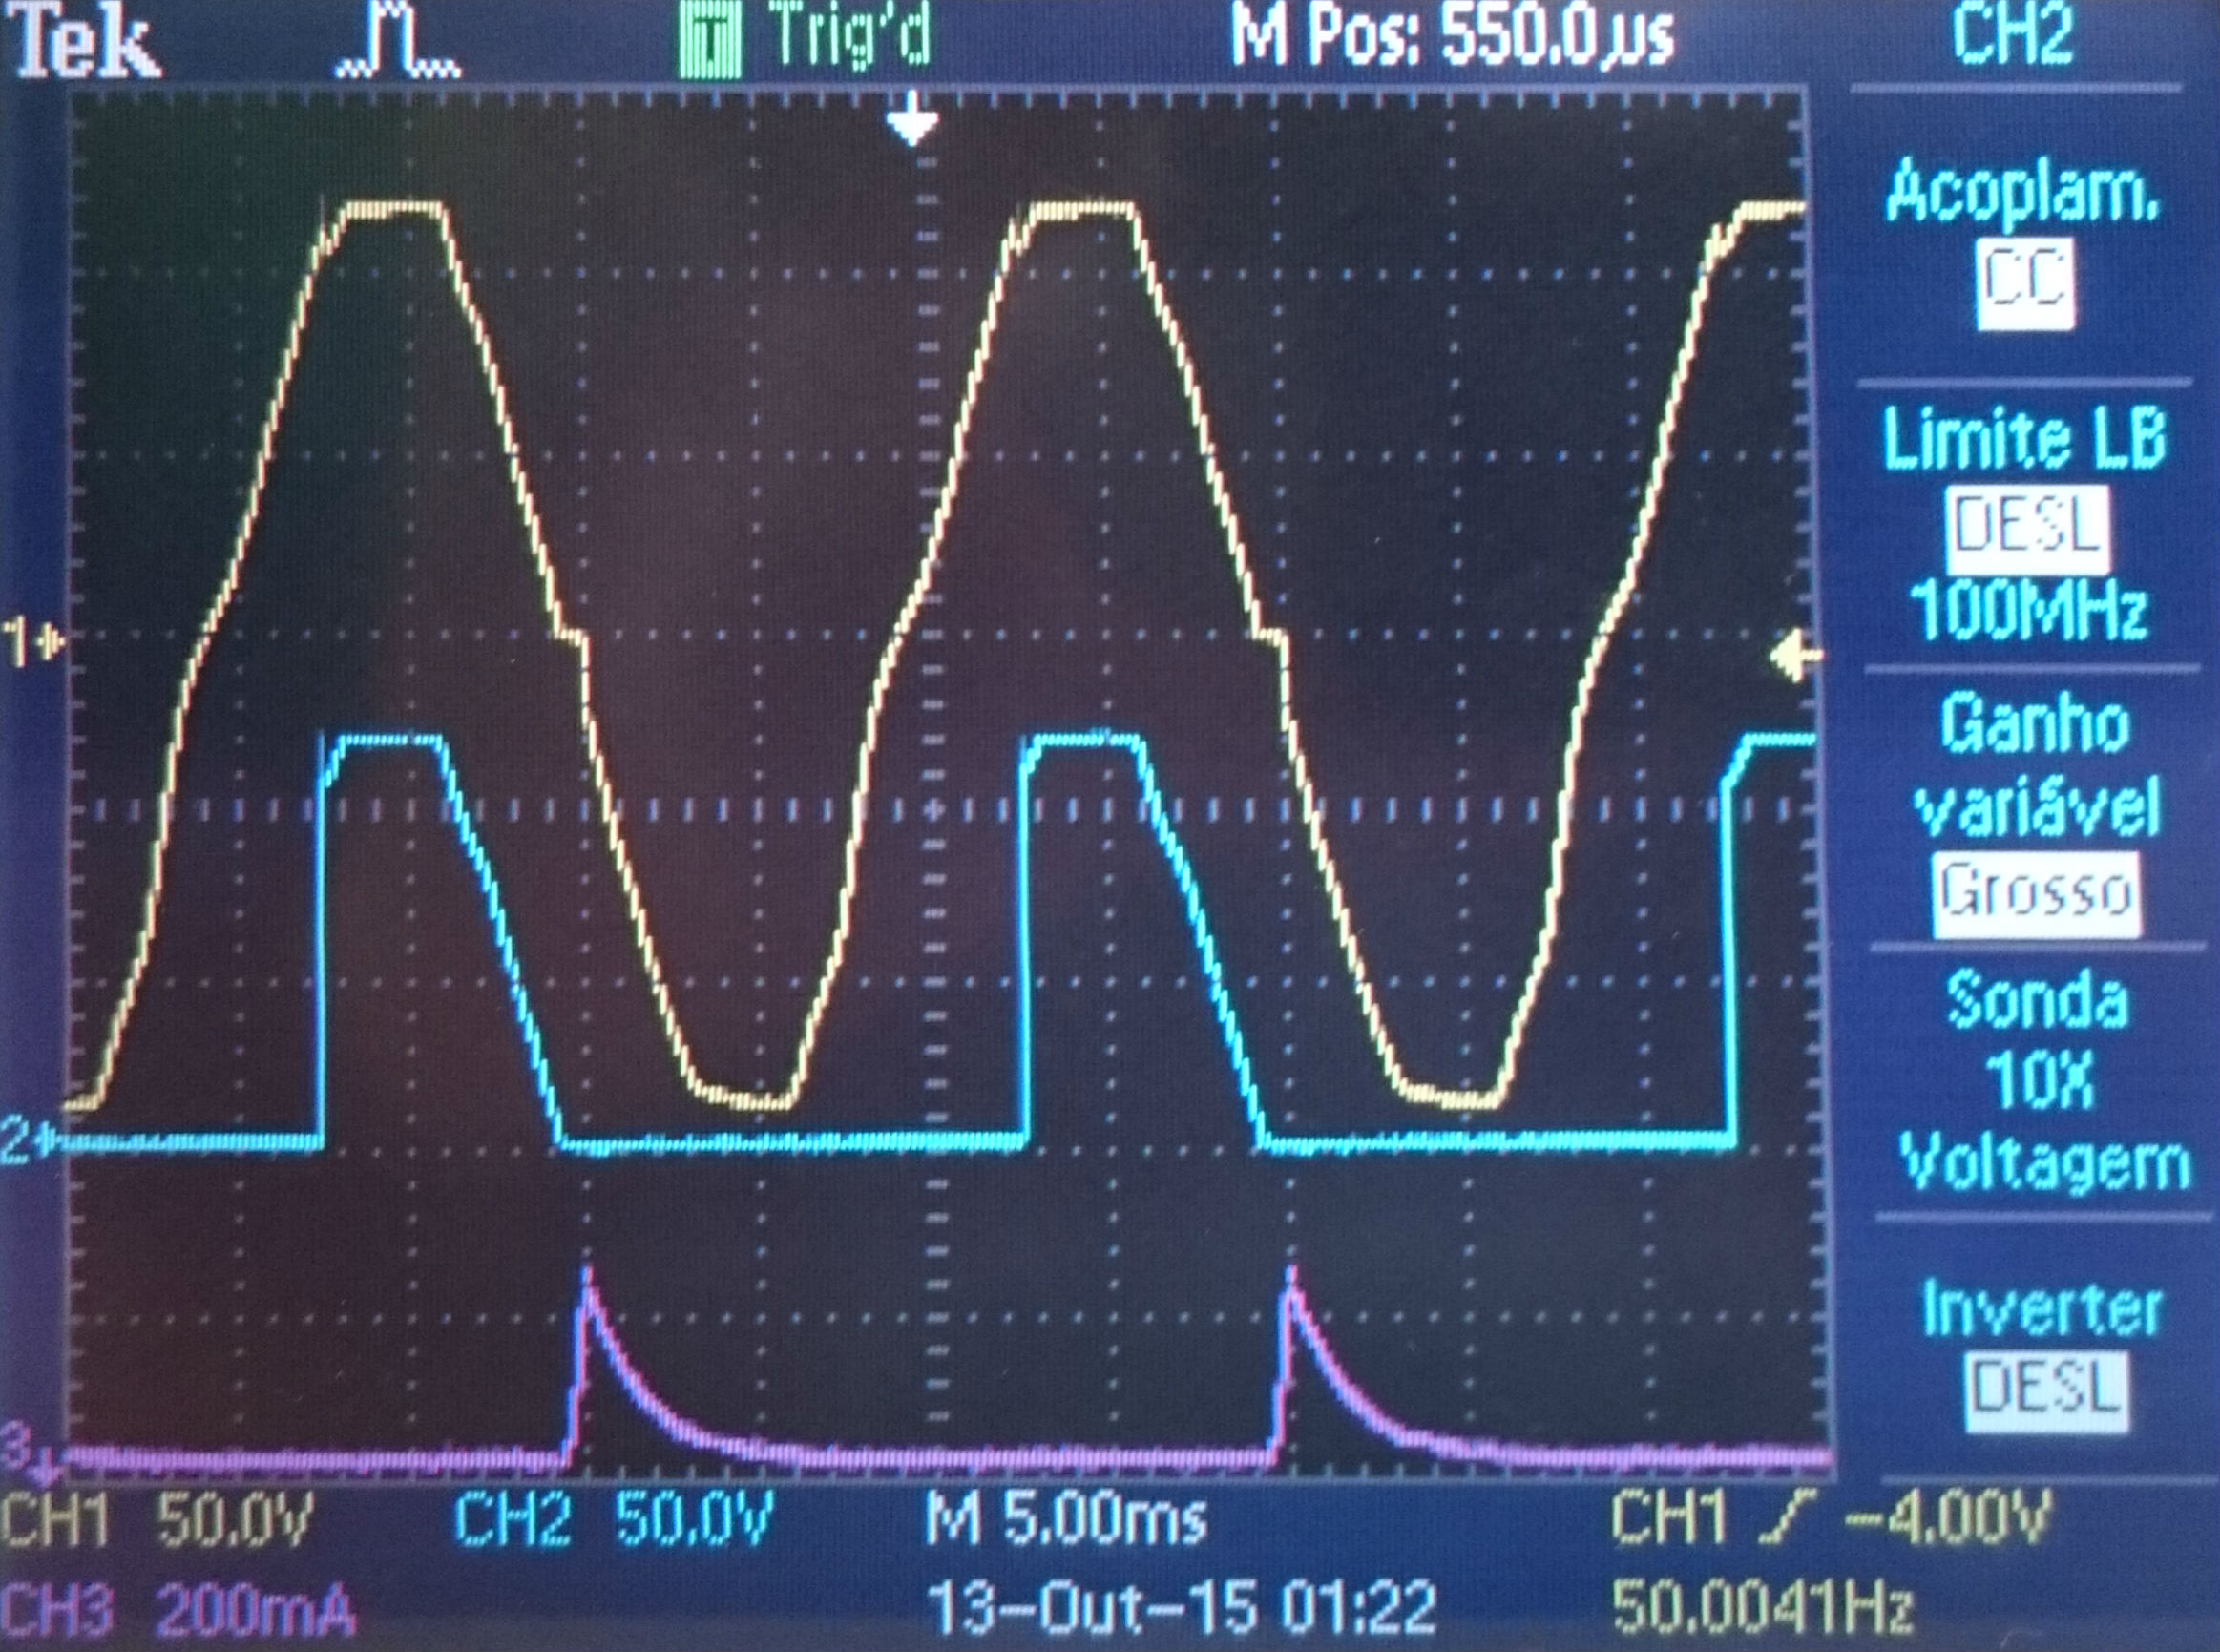
\includegraphics[keepaspectratio=true, scale=0.12]{img/figs/diodo_alfa_dif_zero}
	\caption{Formas de onda de tensão na entrada e corrente no diodo para carga indutiva com $\alpha$ diferente de zero.}
	\label{fig:diodo_alfa_dif_zero}
	\vspace{-0.8em}
\end{figure}

Na \autoref{fig:diodo_alfa_zero} tem-se a tensão na entrada do retificador (a amarelo), a tensão na carga (a azul) e corrente no diodo de roda livre (a rosa) para $\alpha = 0$. Já a \autoref{fig:diodo_alfa_dif_zero} tem-se o comportamento para $\alpha$ diferente de $0$.

Nota-se que a corrente que percorre o díodo é zero até ao momento em que a tensão na carga toma valores negativos. Nesse instante o díodo fica diretamente polarizado e a corrente observável é a de descarga da bobina, que irá decair de forma exponencial até $0$.

\begin{figure}[h]
	\centering
	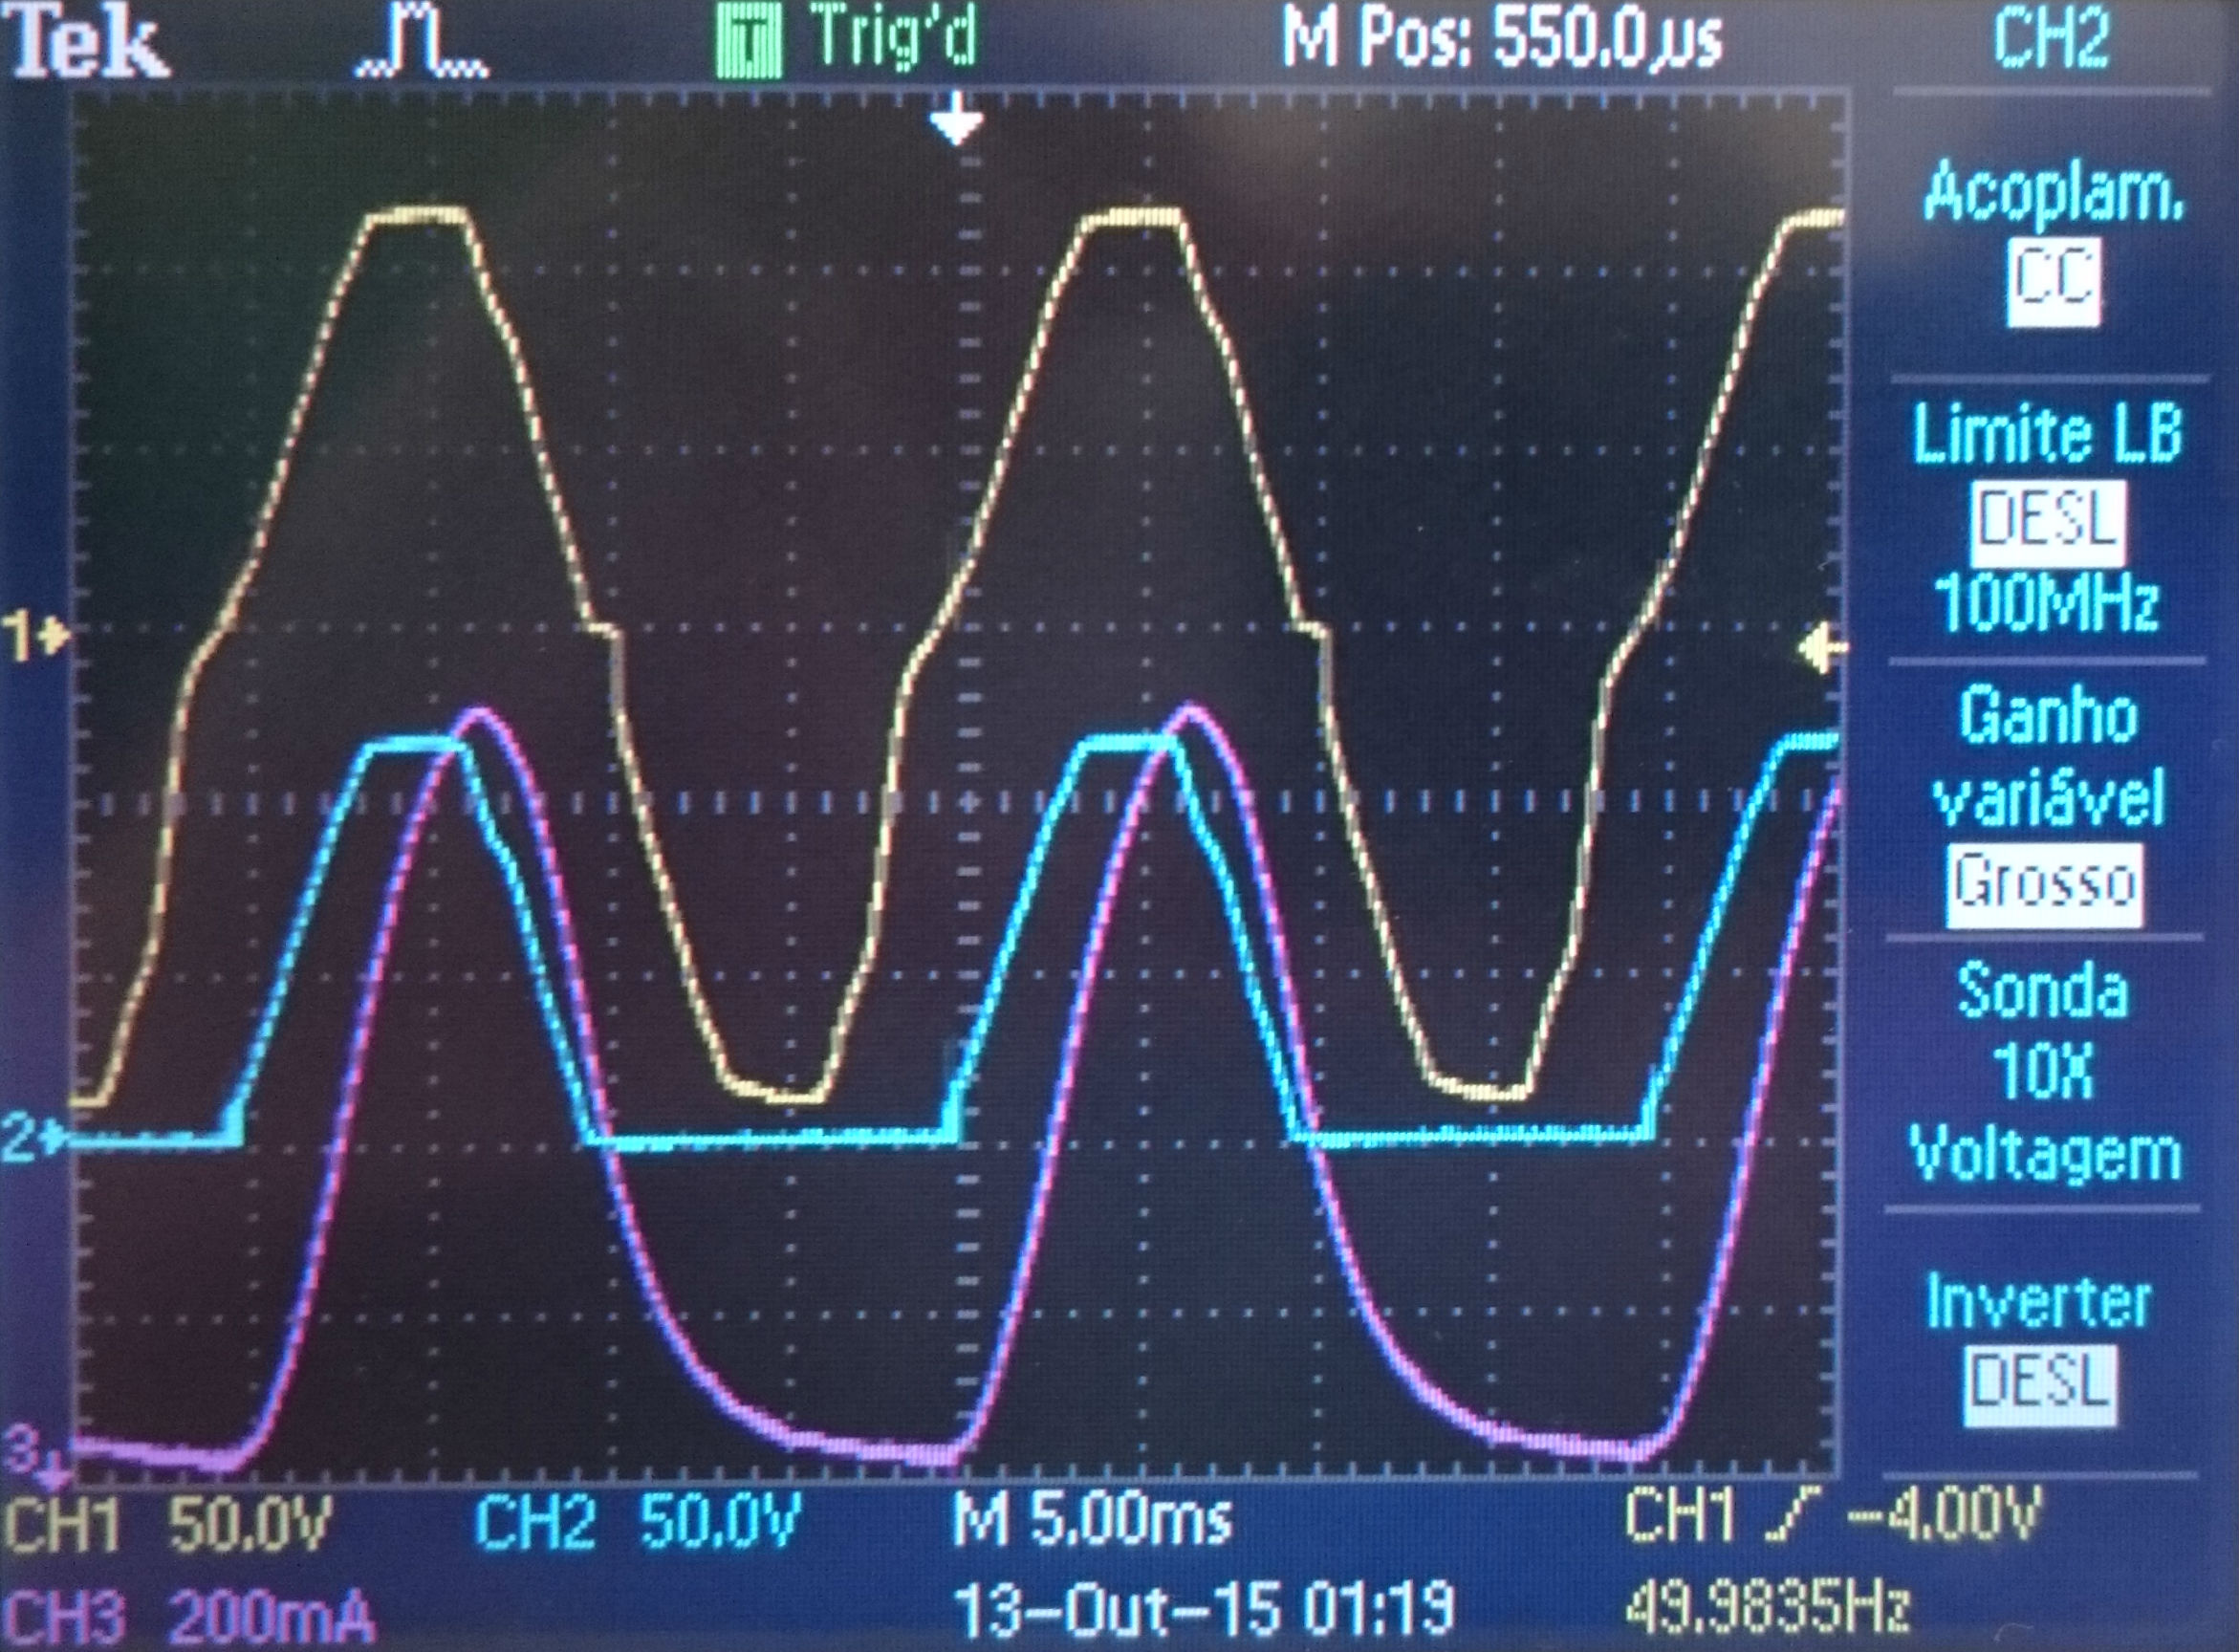
\includegraphics[keepaspectratio=true, scale=0.11]{img/figs/bobine_alfa_zero}
	\caption{Formas de onda da tensão na entrada e corrente na bobina para carga indutiva.}
	\label{fig:bobine_alfa_zero}
	\vspace{-0.8em}
\end{figure}

Na \autoref{fig:bobine_alfa_zero} tem-se a tensão na entrada do retificador (a amarelo), a tensão na carga (a azul) e corrente na bobina (a rosa) para $\alpha = 0$. Na \autoref{fig:bobine_alfa_dif_zero}, presente em \autoref{parag:1}, tem-se o comportamento para $\alpha$ diferente de $0$.

Nota-se que embora a tensão na bobina não tenha sido lida, o seu comportamento é conhecido, devendo ter uma forma tal que o seu valor médio seja nulo. Já a corrente comporta-se tal como para o caso de uma carga indutiva até ao momento em que o díodo entra em condução. Nesse instante a corrente apresenta um comportamento exponencial decrescente; isto é similar ao comportamento da corrente que percorre o díodo de roda livre no mesmo período.

Conhecendo agora o comportamento do circuito observa-se que existem duas fases de funcionamento distintas.

Na primeira tem-se alternância positiva da tensão; o tiristor está diretamente polarizado e conduz assim que haja sinal de disparo, o díodo está inversamente polarizado e a tensão na carga é tal como a de entrada.

A segunda fase corresponde à alternância negativa da tensão de entrada; o díodo de roda livre está diretamente polarizado, sendo percorrido pela corrente da carga, passando ao corte assim que a bobina fique descarregada. Já o tiristor está inversamente polarizado, ficando ao corte assim que a corrente passe por zero

\section{Circuitos de Potência usados}
Neste projeto foi utilizado três circuitos de potência, retificador de meia onde com carga resistiva, com carga \textit{RL} e com carga \textit{RL} e díodo roda livre. 

\begin{figure}[h]
	\centering
	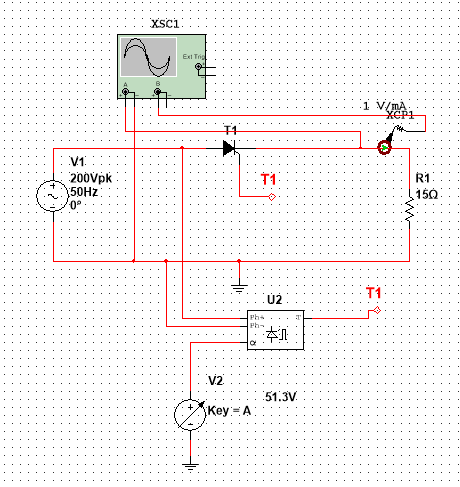
\includegraphics[keepaspectratio=true, scale=0.5]{img/circuito1}
	\caption{Retificador de meia onda com carga resistica, \textit{R}.}
	\label{fig:circuit_3}
	\vspace{-0.8em}
\end{figure}

\begin{figure}[h]
	\centering
	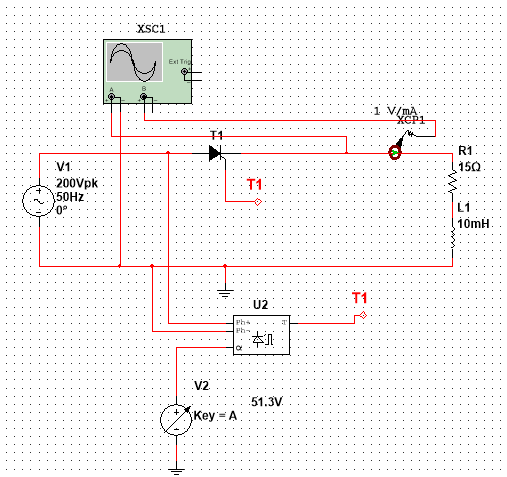
\includegraphics[keepaspectratio=true, scale=0.5]{img/circuito2}
	\caption{Retificador de meia onda com carga \textit{RL}.}
	\label{fig:circuit_4}
	\vspace{-0.8em}
\end{figure}

\begin{figure}[h]
	\centering
	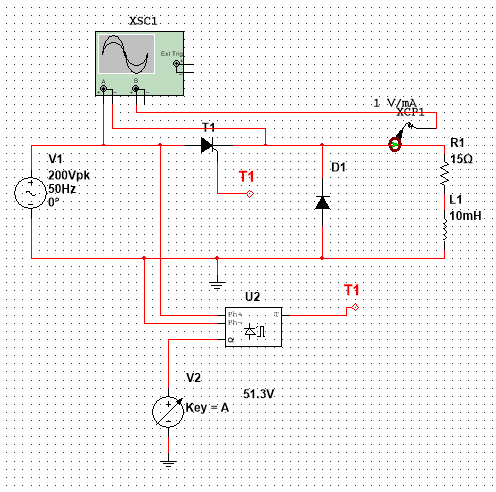
\includegraphics[keepaspectratio=true, scale=0.5]{img/circuito3}
	\caption{Retificador de meia onda com carga \textit{RL} e díodo de roda livre.}
	\label{fig:circuit_5}
	\vspace{-0.8em}
\end{figure}
\pagebreak 

É importante referir que para simulação do circuito de disparos definiu-se que iria ser utilizado um gerador de impulsos com uma frequência   de $50$ Hz, e um \textit{drive} que controla o ângulo de disparo do tiristor uma amplitude de 0 a 5 V. Na \autoref{fig:circuit_6} esta representado o sinal do gerador de impulsos com a tensão de entrada.

\begin{figure}[h]
	\centering
	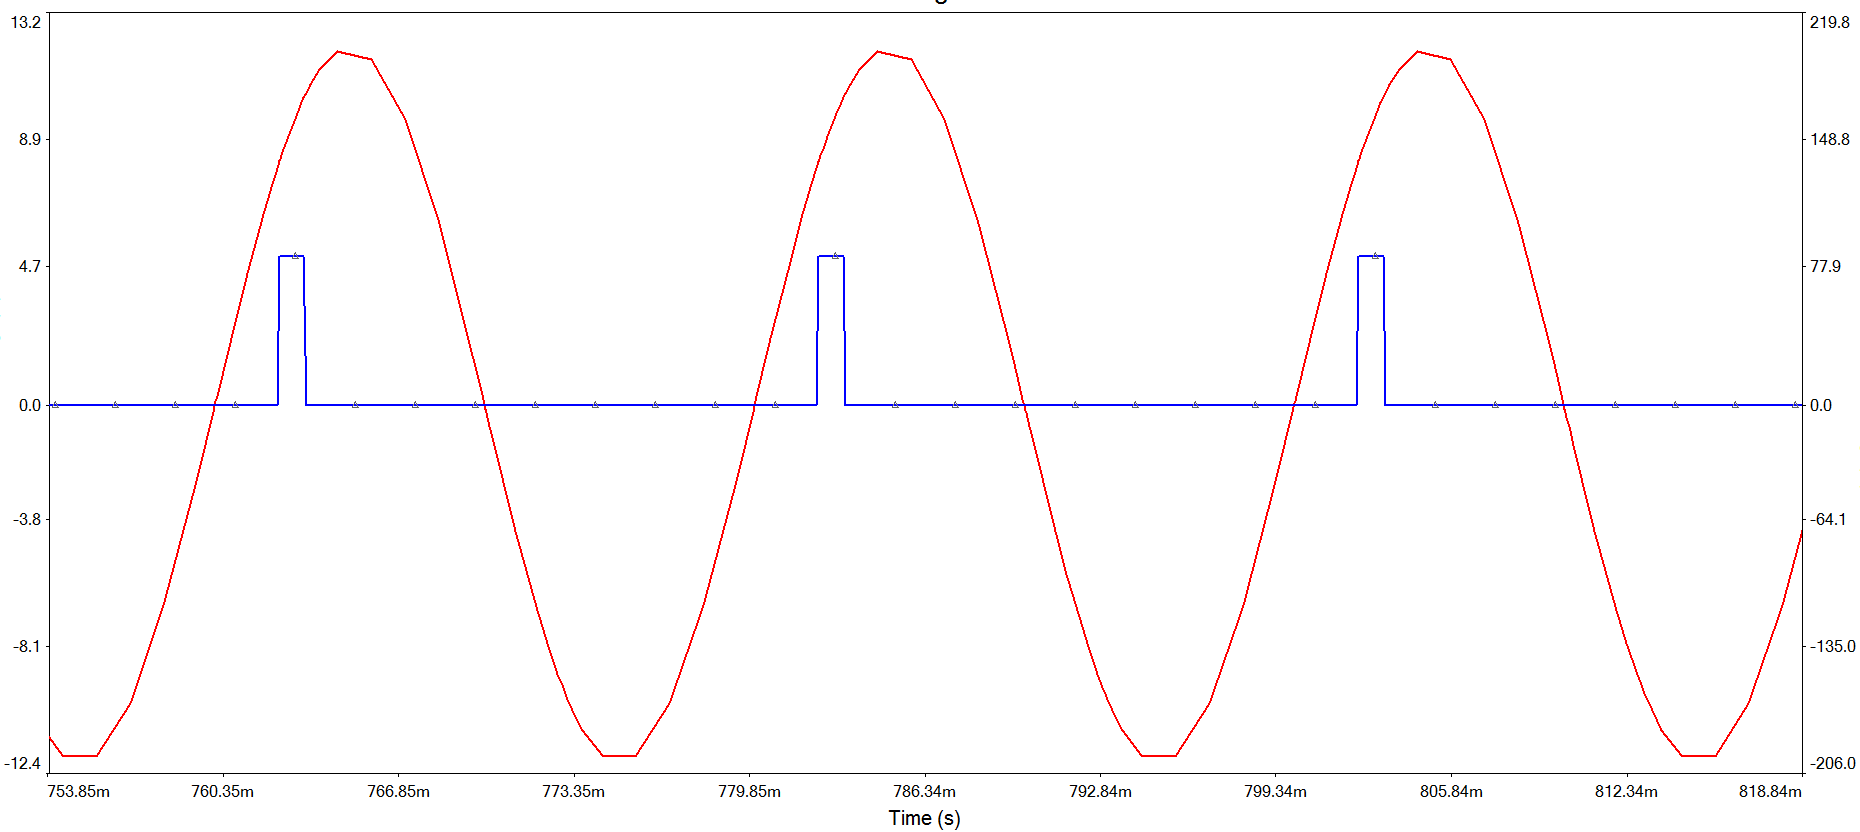
\includegraphics[keepaspectratio=true, scale=0.35]{img/circuito4}
	\caption{Tensão de entrada (a vermelho) e sinal do gerador de impulsos (a azul).}
	\label{fig:circuit_6}
	\vspace{-0.8em}
\end{figure}

\pagebreak
\subsection{Rectificador de meia onda com carga resistiva, \textit{R}}

	Na \autoref{fig:circuit_7}  está representado as formas de onda para a tensão e corrente de entrada.

\begin{figure}[h]
	\centering
	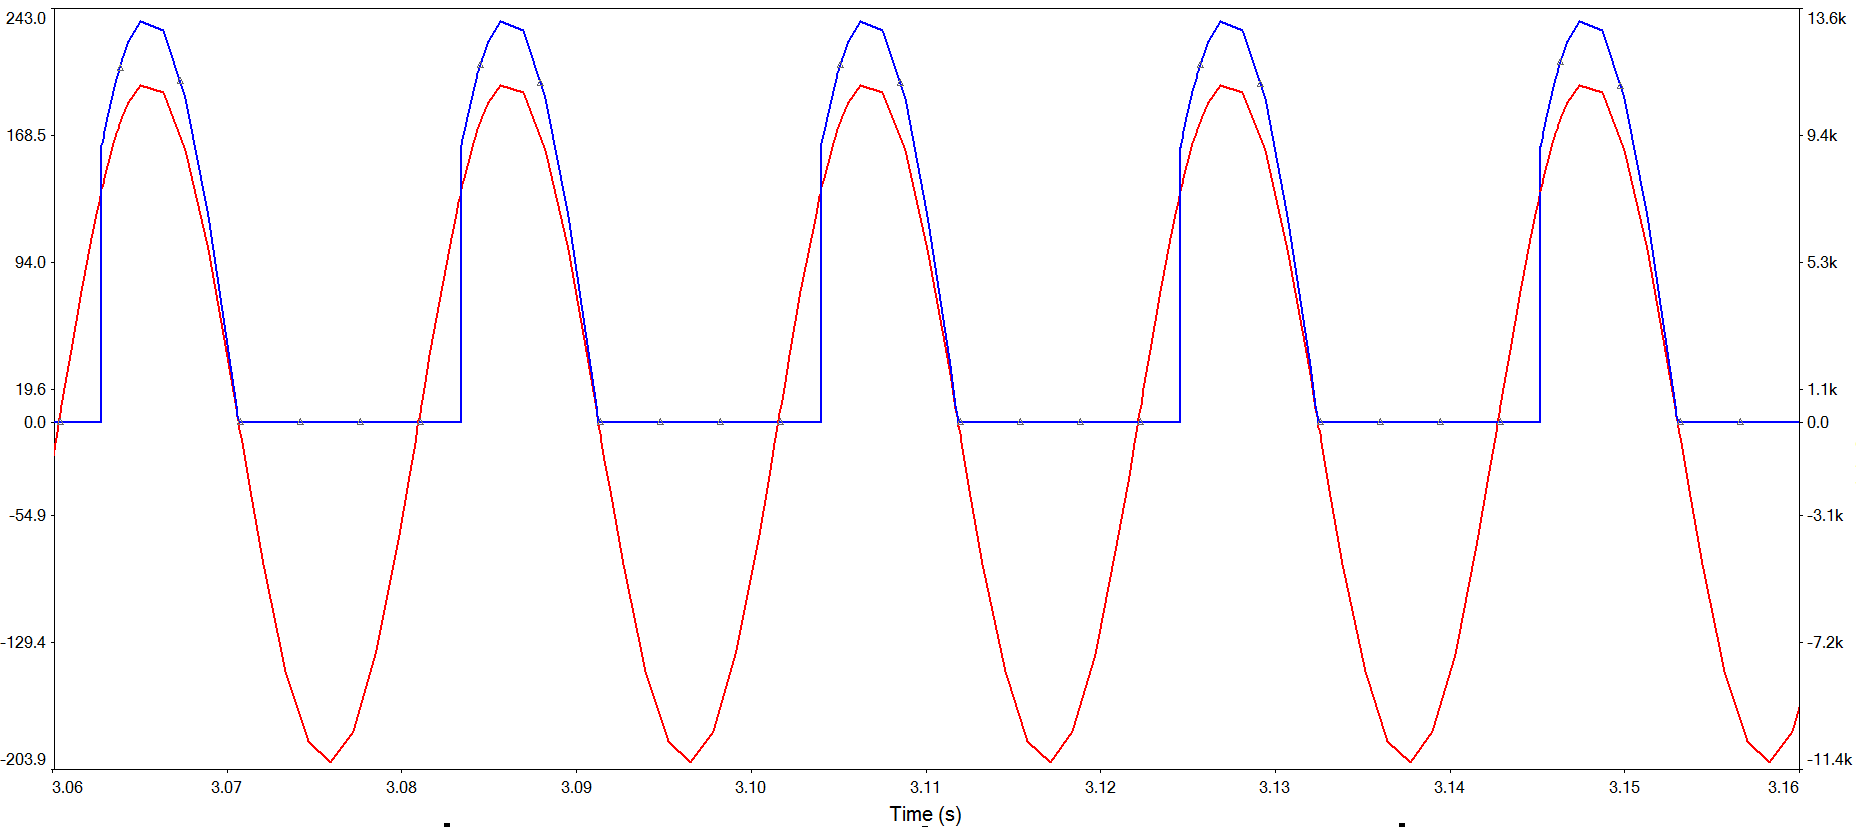
\includegraphics[keepaspectratio=true, scale=0.3]{img/circuito5}
	\caption{Tensão (a vermelho) e corrente (a azul) de entrada.}
	\label{fig:circuit_7}
	\vspace{-0.8em}
\end{figure}

As formas de onda referente a saída do dispositivo podem ser visualizadas na \autoref{fig:circuit_8}.

\begin{figure}[h]
	\centering
	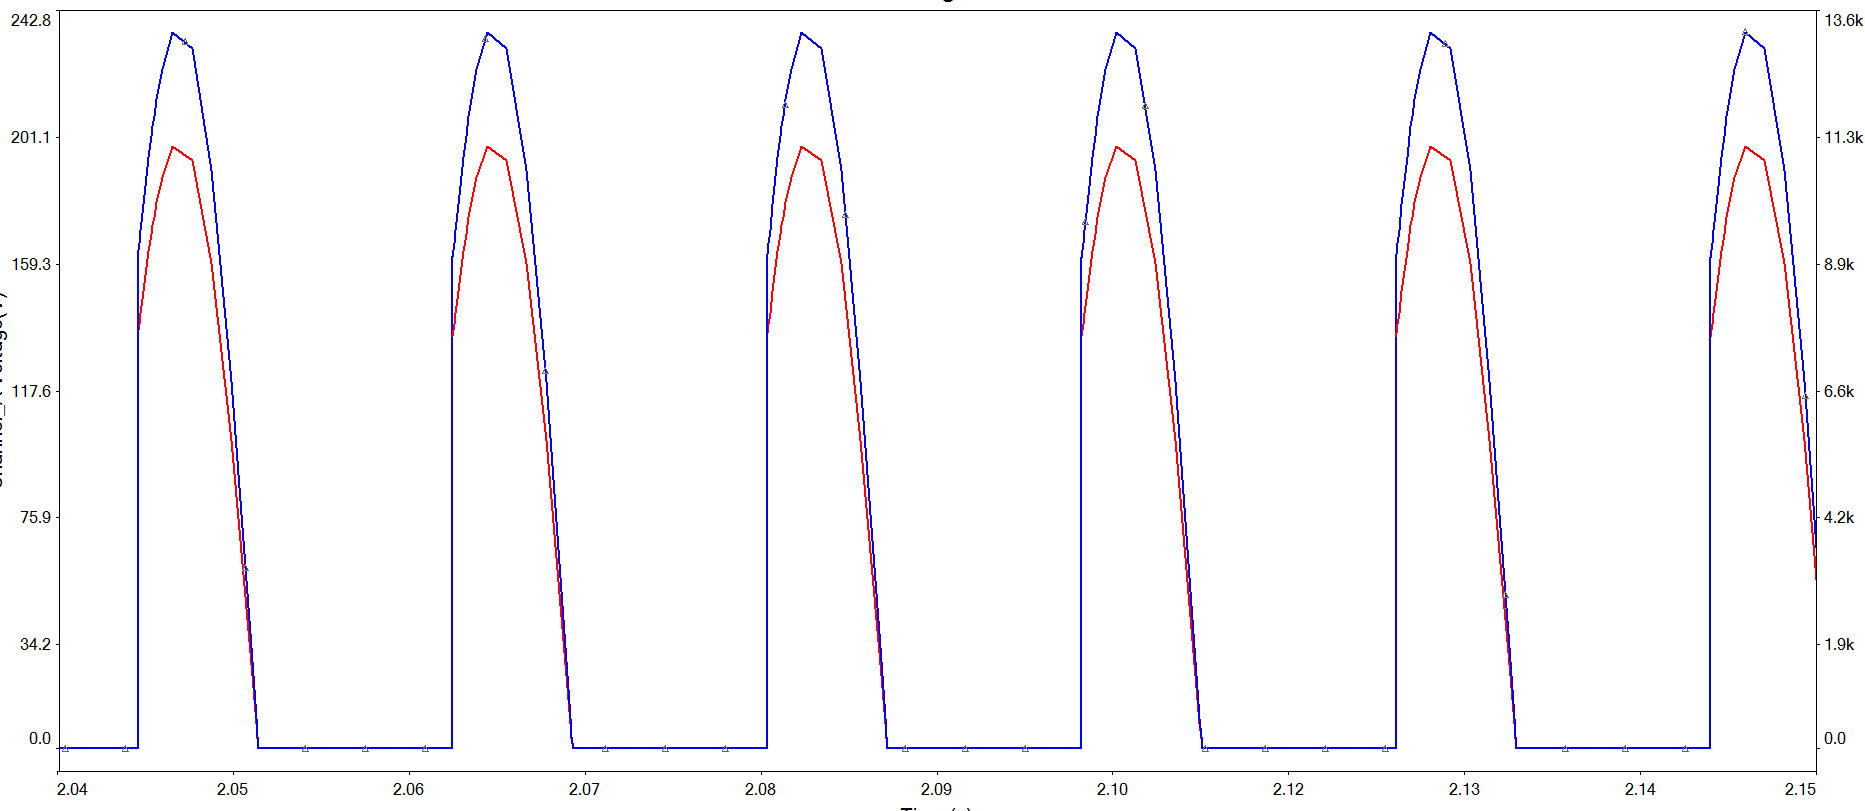
\includegraphics[keepaspectratio=true, scale=0.3]{img/circuito6}
	\caption{Tensão (a vermelho) e corrente (a azul) de saida.}
	\label{fig:circuit_8}
	\vspace{-0.8em}
\end{figure}

Já as formas de onda da tensão e da corrente podem ser visualizadas na  \autoref{fig:circuit_9}.

\begin{figure}[h]
	\centering
	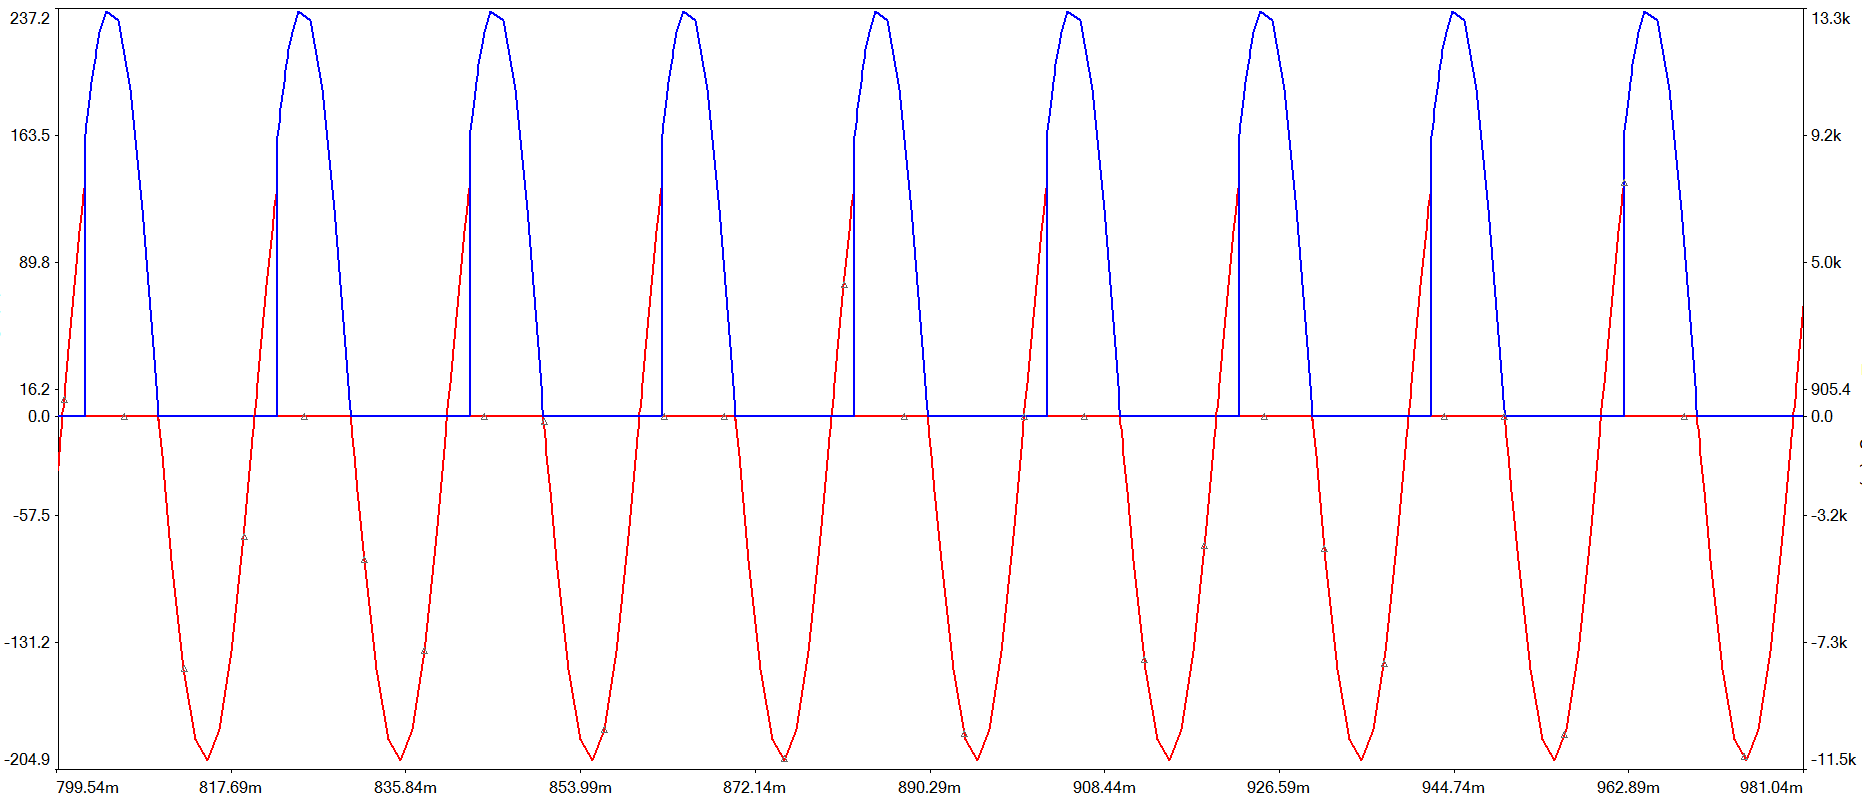
\includegraphics[keepaspectratio=true, scale=0.3]{img/circuito7}
	\caption{Tensão (a vermelho) e corrente (a azul) do tiristor.}
	\label{fig:circuit_9}
	\vspace{-0.8em}
\end{figure}

\pagebreak
\subsection{Rectificador de meia onda com carga \textit{RL}}

De igual forma é importante visualizar o comportamento da tensão e da corrente no dispositivo com uma carga \textit{RL}. É de referir que os sinais à saída estão representados na \autoref{fig:circuit_10} e para o tiristor está representado na \autoref{fig:circuit_11}.

\begin{figure}[h]
	\centering
	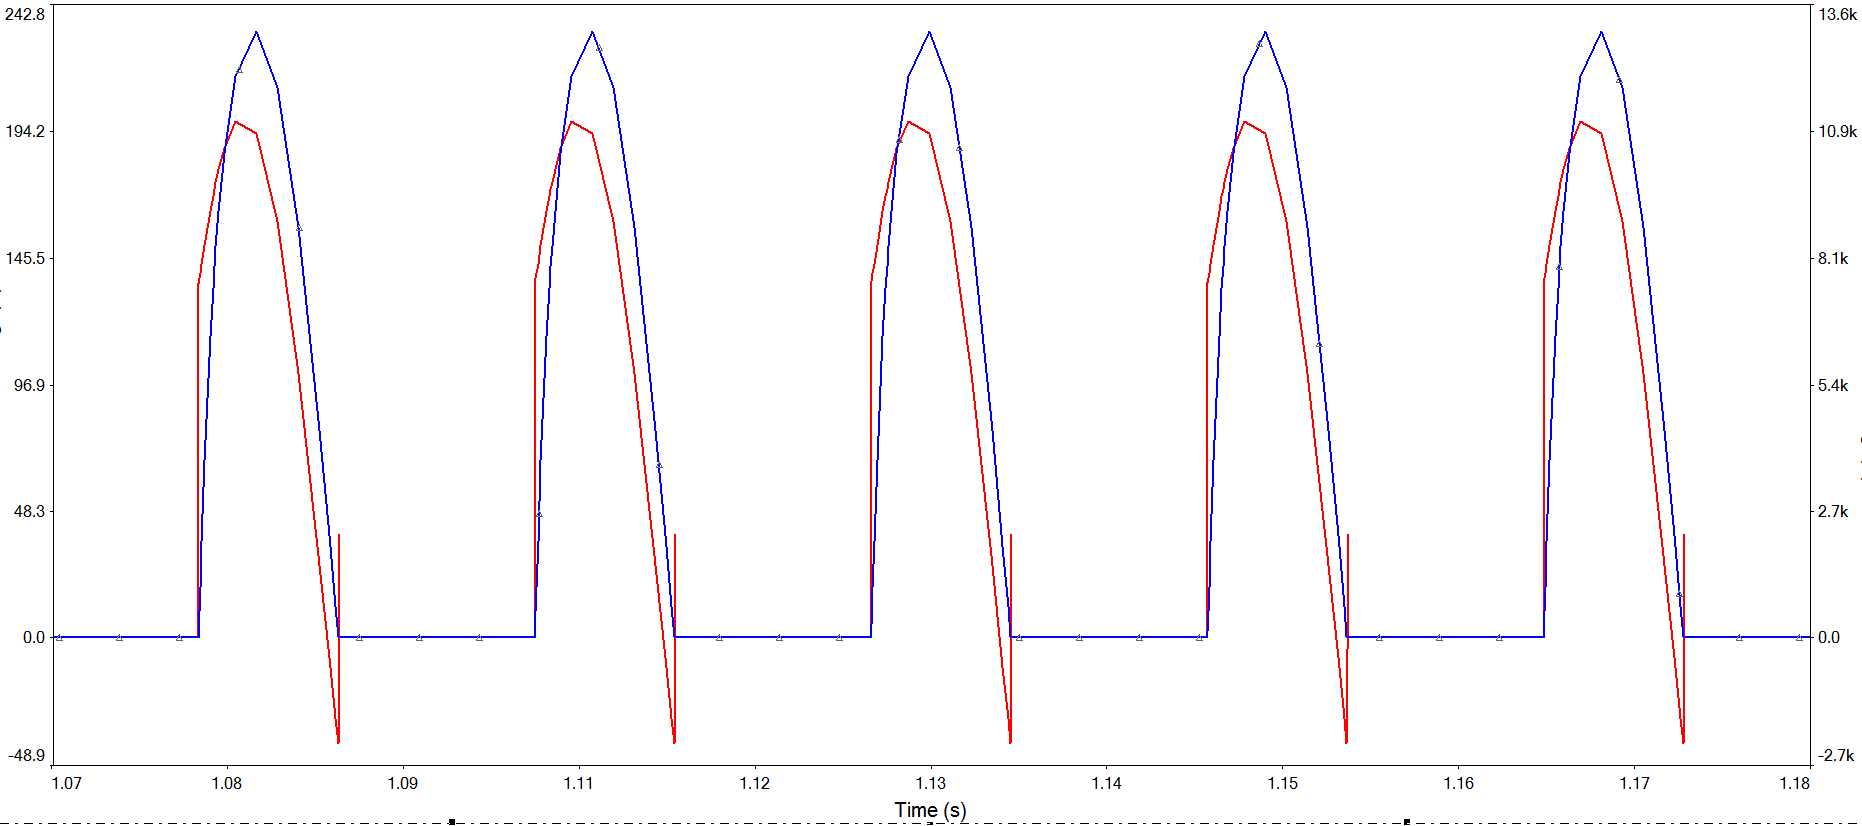
\includegraphics[keepaspectratio=true, scale=0.35]{img/circuito8}
	\caption{Tensão (a vermelho) e corrente (a azul) de saida.}
	\label{fig:circuit_10}
	\vspace{-0.8em}
\end{figure}

\begin{figure}[h]
	\centering
	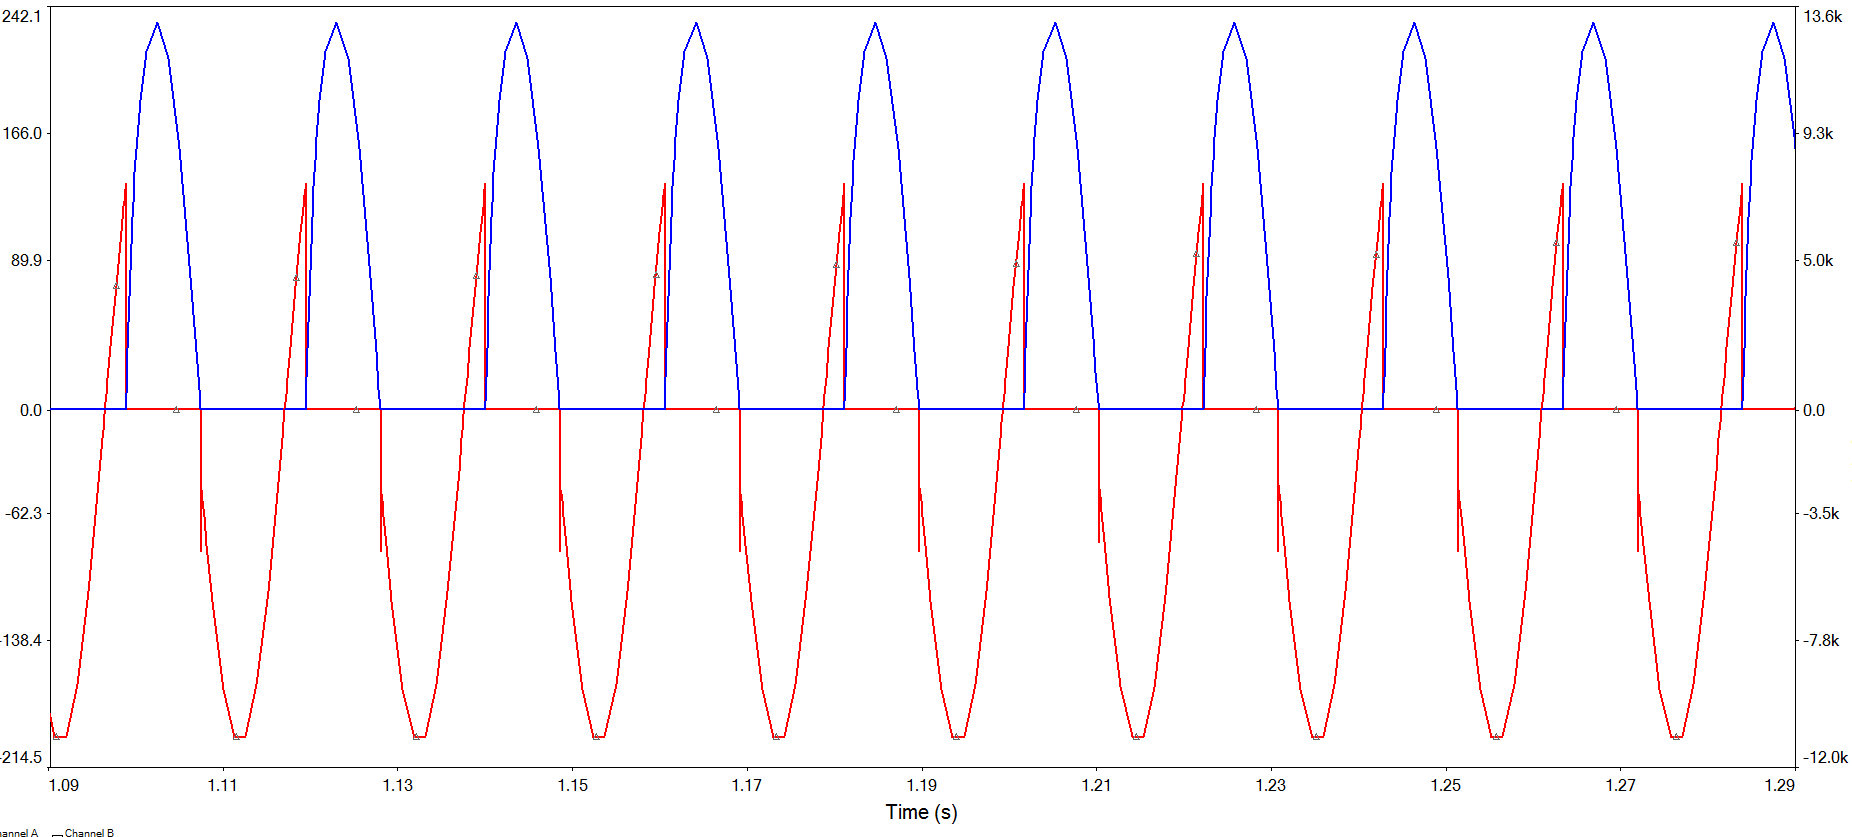
\includegraphics[keepaspectratio=true, scale=0.35]{img/circuito9}
	\caption{Tensão (a vermelho) e corrente (a azul) de tiristor.}
	\label{fig:circuit_11}
	\vspace{-0.8em}
\end{figure}

\subsection{Rectificador de meia onda com carga \textit{RL} e díodo de roda livre}
De igual forma é importante visualizar o comportamento da tensão e da corrente no dispositivo com uma carga \textit{RL} e díodo roda livre. É de referir que os sinais à saída estão representados na \autoref{fig:circuit_12} e para o tiristor está representado na \autoref{fig:circuit_13}.

\begin{figure}[h]
	\centering
	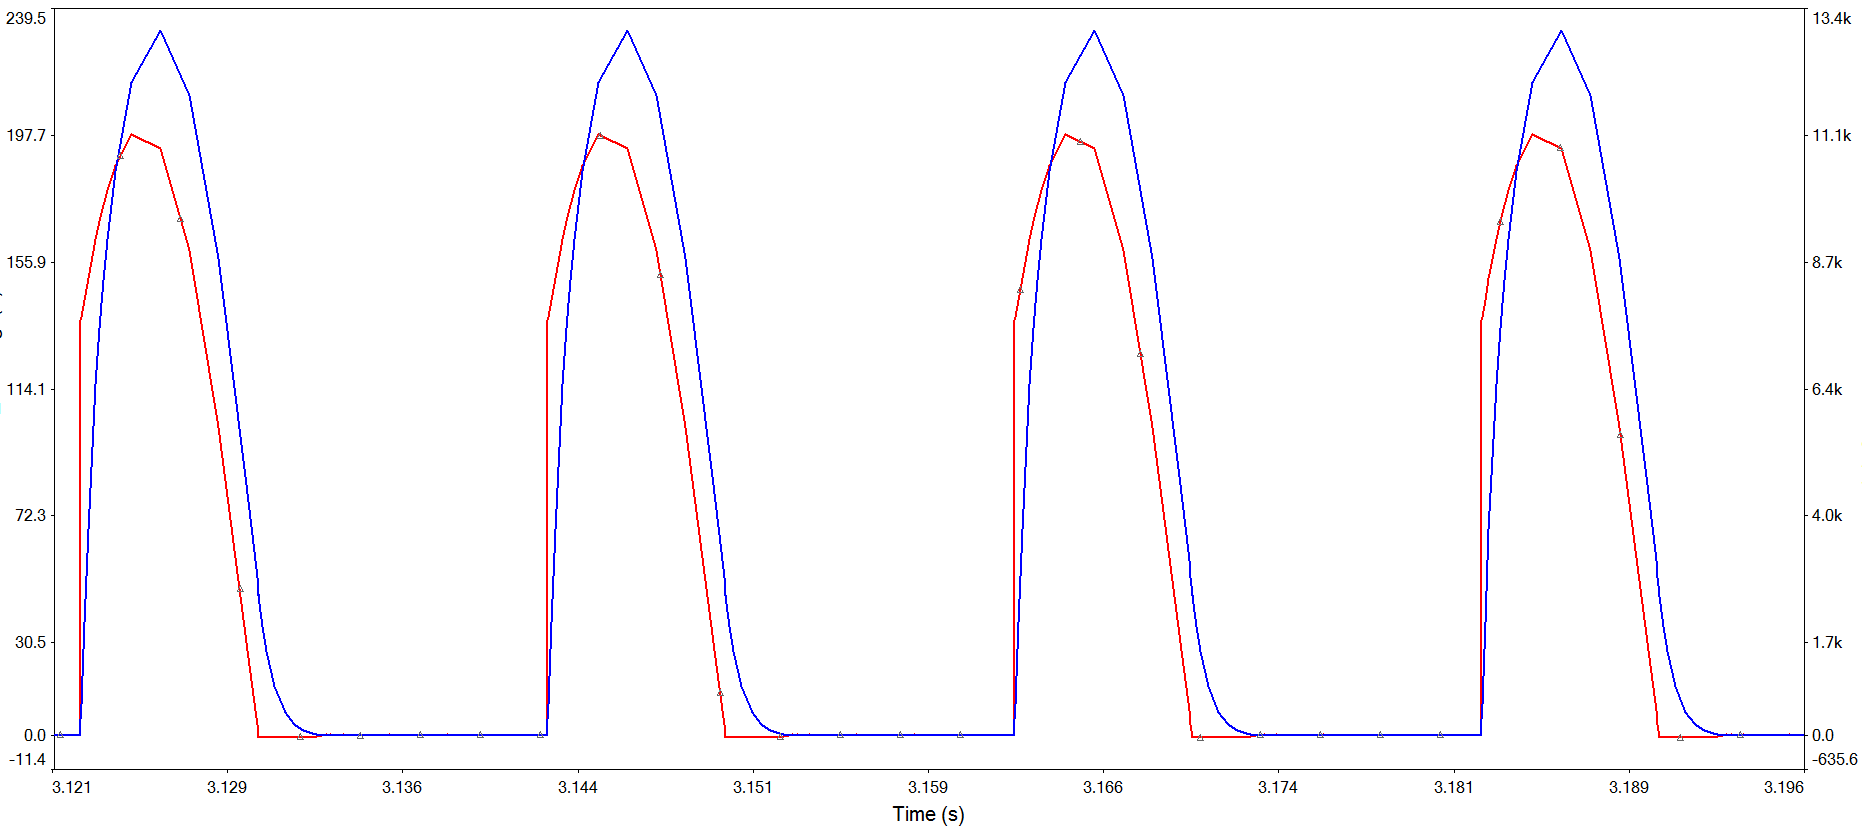
\includegraphics[keepaspectratio=true, scale=0.3]{img/circuito10}
	\caption{Tensão (a vermelho) e corrente (a azul) de saida.}
	\label{fig:circuit_12}
	\vspace{-0.8em}
\end{figure}
\begin{figure}[h]
	\centering
	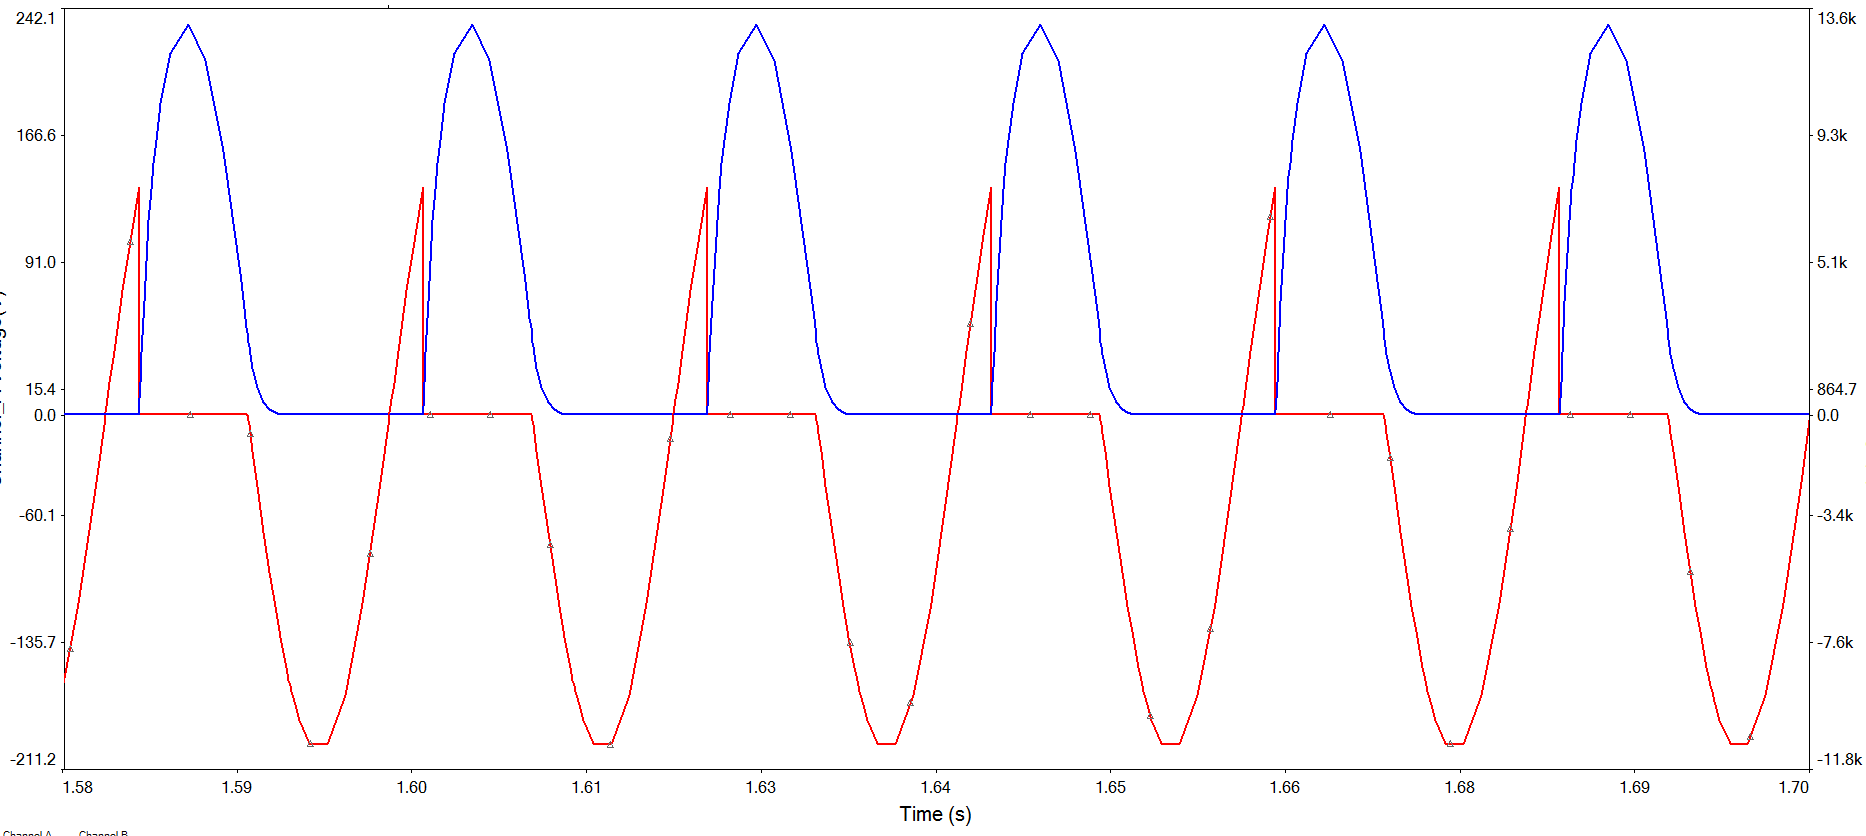
\includegraphics[keepaspectratio=true, scale=0.3]{img/circuito11}
	\caption{Tensão (a vermelho) e corrente (a azul) de tiristor.}
	\label{fig:circuit_13}
	\vspace{-0.8em}
\end{figure}
\pagebreak

Com adição do díodo no circuito é importante visualizar o comportamento da corrente e da tensão neste. Isso pode ser visto na figura \autoref{fig:circuit_14}

\begin{figure}[h]
	\centering
	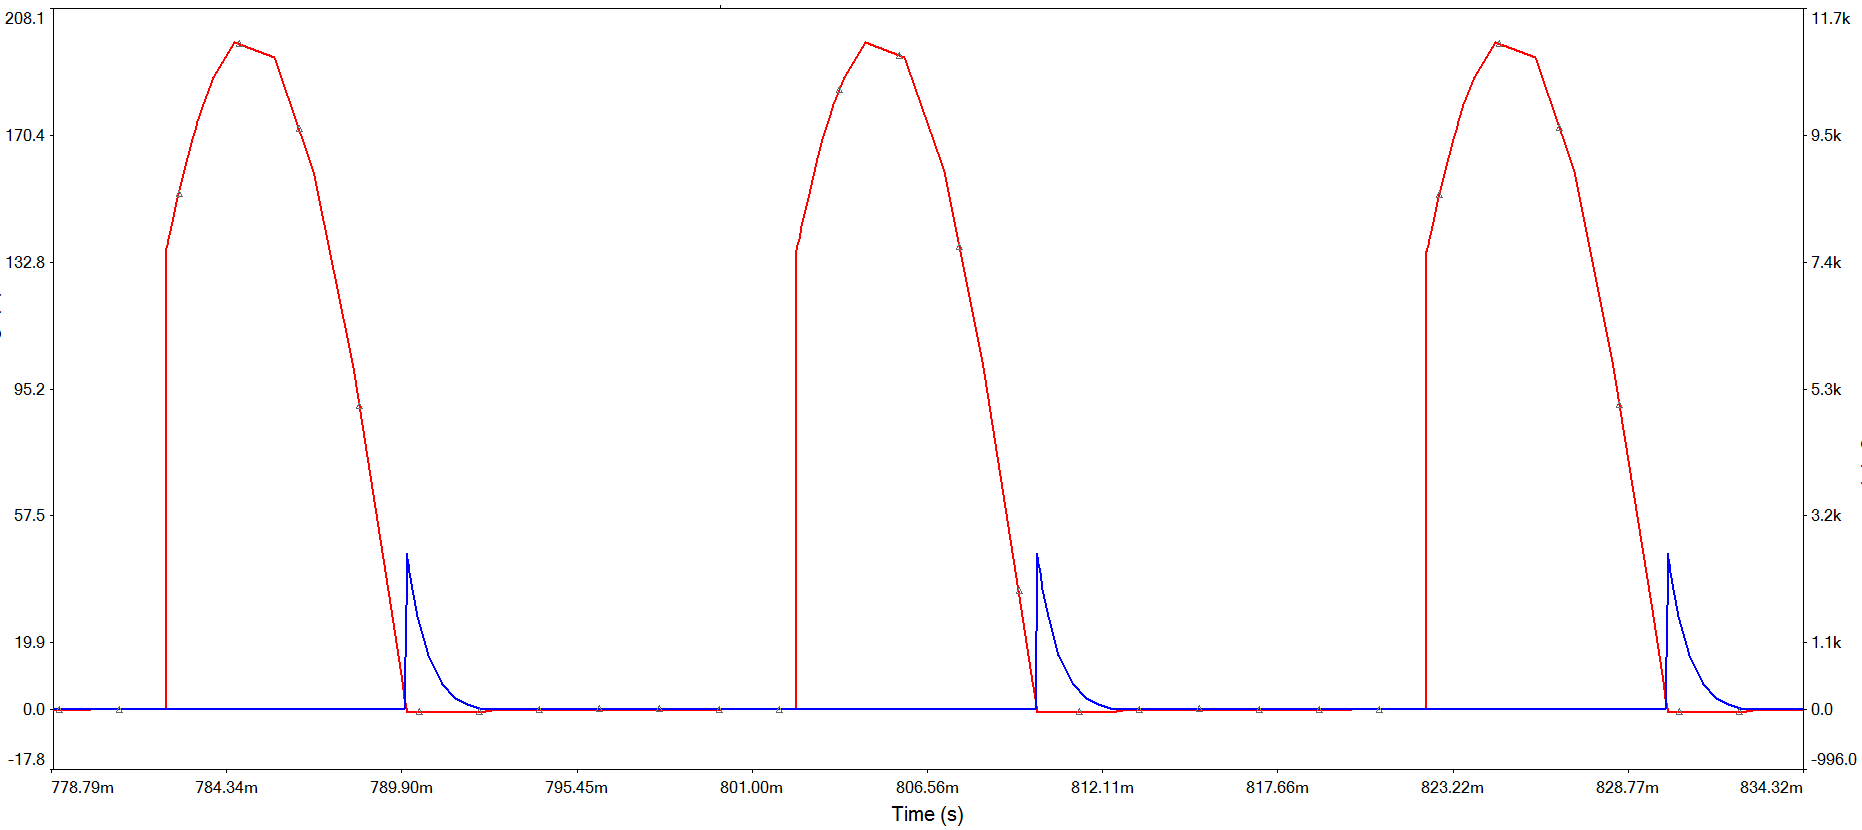
\includegraphics[keepaspectratio=true, scale=0.3]{img/circuito12}
	\caption{Tensão (a vermelho) e corrente (a azul) no díodo de roda livre.}
	\label{fig:circuit_14}
	\vspace{-0.8em}
\end{figure}

\pagebreak

\begin{thebibliography}{2}
	
	\bibitem{Rashid}
	Rashid, Muahammad H. (2004), Power Electronics - Circuits, Devices and Applications, \textit{Prentice Hall}	
	
	\bibitem{Kassakian}
	Kassakian, John G. et al (1992, June), Principles of Power Electronics, \textit{Addison-Wesley Publishing Company}
	
	\bibitem{Silva}
	Silva, Fernando (1998), Eletrónica Industrial, Fundação Calouste Gulbenkian
	
\end{thebibliography}


\pagebreak



\end{document}
